%  LaTeX support: latex@mdpi.compreviously  and CWD 
%  In case you need support, please attach all files that are necessary for compiling as well as the log file, and specify the details of your LaTeX setup (which operating system and LaTeX version / tools you are using).

%=================================================================
%\documentclass[diversity,article,submit,moreauthors,pdftex]{Definitions/mdpi} 
\documentclass[diversity,article,accept,moreauthors,pdftex]{Definitions/mdpi} 
% If you would like to post an early version of this manuscript as a preprint, you may use preprint as the journal and change 'submit' to 'accept'. The document class line would be, e.g., \documentclass[preprints,article,accept,moreauthors,pdftex]{mdpi}. This is especially recommended for submission to arXiv, where line numbers should be removed before posting. For preprints.org, the editorial staff will make this change immediately prior to posting.

%usepackage{showframe}
% Define code chunk aesthetics
\usepackage{listings}
\usepackage{color}

\definecolor{codegreen}{rgb}{0,0.6,0}
\definecolor{codegray}{rgb}{0.5,0.5,0.5}
\definecolor{codepurple}{rgb}{0.58,0,0.82}
\definecolor{backcolour}{RGB}{212,212,212}
\definecolor{bordercolour}{RGB}{0,0,0}

\lstdefinestyle{mystyle}{
    backgroundcolor=\color{backcolour},
    commentstyle=\color{codegreen},
    keywordstyle=\color{magenta},
    numberstyle=\tiny\color{codegray},
    stringstyle=\color{codepurple},
    basicstyle=\ttfamily\footnotesize,
    breakatwhitespace=false,
    breaklines=true,
    captionpos=b,
    keepspaces=true,
    numbers=left,
    numbersep=5pt,
    firstnumber=1,
    showspaces=false,
    showstringspaces=false,
    xleftmargin=9pt,
xrightmargin=3pt,
    showtabs=false,
    tabsize=2,
    frame=single,
    frameround=tttt,
    rulecolor=\color{bordercolour}
}
\lstset{style=mystyle,escapeinside={(*@}{@*)}}


\usepackage[labelformat=simple]{subfig}
\renewcommand\thesubfigure{\normalfont(\textbf{\alph{subfigure}})}  % Compound figures
\usepackage[clean]{revdiff}

%--------------------
% Class Options:
%--------------------
%----------
% journal
%----------
% Choose between the following MDPI journals:
% acoustics, actuators, addictions, admsci, aerospace, agriculture, agriengineering, agronomy, algorithms, animals, antibiotics, antibodies, antioxidants, applsci, arts, asc, asi, atmosphere, atoms, axioms, batteries, bdcc, behavsci , beverages, bioengineering, biology, biomedicines, biomimetics, biomolecules, biosensors, brainsci , buildings, cancers, carbon , catalysts, cells, ceramics, challenges, chemengineering, chemistry, chemosensors, children, cleantechnol, climate, clockssleep, cmd, coatings, colloids, computation, computers, condensedmatter, cosmetics, cryptography, crystals, dairy, data, dentistry, designs , diagnostics, diseases, diversity, drones, econometrics, economies, education, ejihpe, electrochem, electronics, energies, entropy, environments, epigenomes, est, fermentation, fibers, fire, fishes, fluids, foods, forecasting, forests, fractalfract, futureinternet, futurephys, galaxies, games, gastrointestdisord, gels, genealogy, genes, geohazards, geosciences, geriatrics, hazardousmatters, healthcare, heritage, highthroughput, horticulturae, humanities, hydrology, ijerph, ijfs, ijgi, ijms, ijns, ijtpp, informatics, information, infrastructures, inorganics, insects, instruments, inventions, iot, j, jcdd, jcm, jcp, jcs, jdb, jfb, jfmk, jimaging, jintelligence, jlpea, jmmp, jmse, jnt, jof, joitmc, jpm, jrfm, jsan, land, languages, laws, life, literature, logistics, lubricants, machines, magnetochemistry, make, marinedrugs, materials, mathematics, mca, medicina, medicines, medsci, membranes, metabolites, metals, microarrays, micromachines, microorganisms, minerals, modelling, molbank, molecules, mps, mti, nanomaterials, ncrna, neuroglia, nitrogen, notspecified, nutrients, ohbm, optics, particles, pathogens, pharmaceuticals, pharmaceutics, pharmacy, philosophies, photonics, physics, plants, plasma, polymers, polysaccharides, preprints , proceedings, processes, proteomes, psych, publications, quantumrep, quaternary, qubs, reactions, recycling, religions, remotesensing, reports, resources, risks, robotics, safety, sci, scipharm, sensors, separations, sexes, signals, sinusitis, smartcities, sna, societies, socsci, soilsystems, sports, standards, stats, surfaces, surgeries, sustainability, symmetry, systems, technologies, test, toxics, toxins, tropicalmed, universe, urbansci, vaccines, vehicles, vetsci, vibration, viruses, vision, water, wem, wevj

%---------
% article
%---------
% The default type of manuscript is "article", but can be replaced by: 
% abstract, addendum, article, benchmark, book, bookreview, briefreport, casereport, changes, comment, commentary, communication, conceptpaper, conferenceproceedings, correction, conferencereport, expressionofconcern, extendedabstract, meetingreport, creative, datadescriptor, discussion, editorial, essay, erratum, hypothesis, interestingimages, letter, meetingreport, newbookreceived, obituary, opinion, projectreport, reply, retraction, review, perspective, protocol, shortnote, supfile, technicalnote, viewpoint
% supfile = supplementary materials
\setitemize{parsep=6pt,itemsep=0pt,leftmargin=*,labelsep=5.5mm}
\setenumerate{parsep=6pt,itemsep=0pt,leftmargin=*,labelsep=5.5mm}
\setlist[description]{itemsep=0mm}

%----------
% submit
%----------
% The class option "submit" will be changed to "accept" by the Editorial Office when the paper is accepted. This will only make changes to the frontpage (e.g., the logo of the journal will get visible), the headings, and the copyright information. Also, line numbering will be removed. Journal info and pagination for accepted papers will also be assigned by the Editorial Office.

%------------------
% moreauthors
%------------------
% If there is only one author the class option oneauthor should be used. Otherwise use the class option moreauthors.

%---------
% pdftex
%---------
% The option pdftex is for use with pdfLaTeX. If eps figures are used, remove the option pdftex and use LaTeX and dvi2pdf.

%=================================================================
\firstpage{1} 
\makeatletter 
\setcounter{page}{\@firstpage} 
\makeatother
\pubvolume{12}
\issuenum{4}
\articlenumber{0}
\pubyear{2020}
\copyrightyear{2020}
%\externaleditor{Academic Editor: name}
\history{Received: date; Accepted: date; Published: date}
\updates{yes} % If there is an update available, un-comment this line

%% MDPI internal command: uncomment if new journal that already uses continuous page numbers 
%\continuouspages{yes}

%------------------------------------------------------------------
% The following line should be uncommented if the LaTeX file is uploaded to arXiv.org
%\pdfoutput=1

%=================================================================
% Add packages and commands here. The following packages are loaded in our class file: fontenc, calc, indentfirst, fancyhdr, graphicx, lastpage, ifthen, lineno, float, amsmath, setspace, enumitem, mathpazo, booktabs, titlesec, etoolbox, amsthm, hyphenat, natbib, hyperref, footmisc, geometry, caption, url, mdframed, tabto, soul, multirow, microtype, tikz
\usepackage{xcolor}
\newcommand{\todo}[1]{\textcolor{red}{\textbf{#1}}}   % \todo{NOTE TO SELF WRITTEN IN RED}

%=================================================================
%% Please use the following mathematics environments: Theorem, Lemma, Corollary, Proposition, Characterization, Property, Problem, Example, ExamplesandDefinitions, Hypothesis, Remark, Definition, Notation, Assumption
%% For proofs, please use the proof environment (the amsthm package is loaded by the MDPI class).

%=================================================================
% Full title of the paper (Capitalized)
\Title{Diversity and Structure of an Arid Woodland in Southwest Angola, with Comparison to the Wider Miombo Ecoregion}

%Attention AE/ME. The following layout issues have not been checked by the English Editing Department and must be carefully verified by the AE/Layout Department: All callout issues, bold usage of callouts, and references to callouts in the text. Correct callout usage in figures. Figure and Table layout issues. Footnote formatting and Glossaries have not been checked. En dash usage for negative values, en dash usage to indicate relationships, en dash usage to indicate bonds (especially in chemistry). The English Editing Department is not responsible for correct italic usage for genes, proteins and technical terminology. This responsibility belongs to the authors. The following are also not checked: spacing between numbers and units of measurement, ratios, en dashes for ranges, date and time formats, punctuation in equation lines, and less than/more than spacing (< >). Finally, capitalization and layout of titles/headings must be properly checked as well as ensuring 'Eq.' and 'Fig.' are properly spelled out, as these are layout issues.

% Author Orchid ID: enter ID or remove command
\newcommand{\orcidauthorA}{0000-0001-5595-255X} % John Godlee 
\newcommand{\orcidauthorB}{0000-0002-8859-7491} % Francisco Maiato
\newcommand{\orcidauthorC}{0000-0002-3770-2482} % Jose Tchamba 
\newcommand{\orcidauthorD}{0000-0002-5137-1448} % Valter Chisingui 
% \newcommand{\orcidauthorE}{} % Jonathan Muledi
\newcommand{\orcidauthorF}{0000-0003-3208-5443} % Mylor Shutcha 
\newcommand{\orcidauthorH}{0000-0002-1802-0128} % Casey Ryan 
\newcommand{\orcidauthorI}{0000-0001-9232-5221} % Kyle Dexter
\newcommand{\orcidauthorJ}{0000-0002-4852-7085} % Thom Brade

% Authors, for the paper (add full first names)
\Author{\hl{John L. Godlee} %Please carefully check the accuracy of names and affiliations. Changes will not be possible after proofreading.
 $^{1,}$*\orcidA{}, Francisco Maiato Gon\c{c}alves $^{2}$\orcidB{}, Jos\'{e} Jo\~{a}o Tchamba $^{2}$\orcidC{}, \mbox{Antonio Valter Chisingui $^{2}$\orcidD{}}, Jonathan Ilunga Muledi $^{3}$, Mylor Ngoy Shutcha $^{3}$\orcidF{}, \mbox{Casey M. Ryan $^{1}$\orcidH{}}, Thom K. Brade $^{1}$\orcidJ{} and Kyle G. Dexter $^{1,4}$\orcidI{}}

% Authors, for metadata in PDF
\AuthorNames{John L. Godlee, Francisco Maiato Goncalves, Jos\'{e} Jo\~{a}o Tchamba,  Antonio Valter Chisingui, Jonathan Ilunga Muledi, Mylor Ngoy Shutcha, Casey M. Ryan, Thom K. Brade and Kyle G. Dexter}

% Affiliations / Addresses (Add [1] after \address if there is only one affiliation.)
\address{%
$^{1}$ \quad School of GeoSciences, University of Edinburgh, \hl{Edinburgh}, EH93FF, UK; \hl{casey.ryan@ed.ac.uk (C.M.R.); Thom.Brade@ed.ac.uk (T.K.B.); kyle.dexter@ed.ac.uk (K.G.D.)}\\ %Please add the post code. We added e-mails from redmine, please confirm.
$^{2}$ \quad Herbarium of Lubango, ISCED Hu\'{i}la, Sarmento Rodrigues Str. No. 2, CP. 230, \hl{Lubango}, Angola; \hl{francisco.maiato@gmail.com (F.M.G.); tchamba417@gmail.com (J.J.T.); vachissingui@gmail.com (A.V.C.)}\\%Please add the post code.
$^{3}$ \quad Ecologie, Restauration Ecologique et Paysage, Facult\'{e} des Sciences Agronomique, Universit\'{e}~de~Lubumbashi, Route Kasapa BP 1825, Congo; \hl{jonathanmuledi@gmail.com (J.I.M.); mylorshutcha@gmail.com~(M.N.S.)}\\
$^{4}$ \quad Royal Botanic Garden Edinburgh, Edinburgh EH3 5LR, UK}

% Contact information of the corresponding author
\corres{Correspondence: johngodlee@gmail.com}

% Current address and/or shared authorship
%\firstnote{Current address: Crew Building, The King's Buildings, Edinburgh, EH9 3FF, United Kingdom} % \dagger
% The commands \thirdnote{} till \eighthnote{} are available for further notes

%\simplesumm{} % Simple summary

%\conference{} % An extended version of a conference paper

% Abstract (Do not insert blank lines, i.e. \\) 
% 200 words max
% (1) Background: Place the question addressed in a broad context and highlight the purpose of the study; 
% (2) Methods: Describe briefly the main methods or treatments applied; 
% (3) Results: Summarize the article's main findings; and 
% (4) Conclusion: Indicate the main conclusions or interpretations. 
% The abstract should be an objective representation of the article, it must not contain results which are not presented and substantiated in the main text and should not exaggerate the main conclusions.
\abstract{Seasonally dry woodlands are the dominant land cover across southern Africa. They~are biodiverse, structurally complex, and important for ecosystem service provision. Species composition and structure vary across the region producing a diverse array of woodland types. The woodlands of the Hu\'{i}la plateau in southwest Angola represent the extreme southwestern extent of the miombo ecoregion and are markedly drier than other woodlands within this ecoregion. They~remain understudied, however, compared to woodlands further east in the miombo ecoregion. We~aimed to elucidate further the tree diversity found within southwestern Angolan woodlands by conducting a plot-based study in Bicuar National Park, comparing tree species composition and woodland structure with similar plots in Tanzania, Mozambique, and the Democratic Republic of Congo. We~found Bicuar National Park had comparatively low tree species diversity, but contained 27 tree species not found in other plots. Plots in Bicuar had low basal area, excepting plots dominated by \textit{Baikiaea plurijuga}. In a comparison of plots in intact vegetation with areas previously disturbed by shifting-cultivation agriculture, we found species diversity was marginally higher in disturbed plots. Bicuar National Park remains an important woodland refuge in Angola, with an uncommon mosaic of woodland types within a small area. While we highlight wide variation in species composition and woodland structure across the miombo ecoregion, plot-based studies with more dense sampling across the ecoregion are clearly needed to more broadly understand regional variation in vegetation diversity, composition and structure.}

% Keywords
% 3-10
\keyword{woodland, miombo, savanna, diversity, disturbance, Baikiaea}

% The fields PACS, MSC, and JEL may be left empty or commented out if not applicable
%\PACS{J0101}
%\MSC{}
%\JEL{}

%%%%%%%%%%%%%%%%%%%%%%%%%%%%%%%%%%%%%%%%%%
% Only for the journal Diversity
%\LSID{\url{http://}}

%%%%%%%%%%%%%%%%%%%%%%%%%%%%%%%%%%%%%%%%%%
% Only for the journal Applied Sciences:
%\featuredapplication{Authors are encouraged to provide a concise description of the specific application or a potential application of the work. This section is not mandatory.}
%%%%%%%%%%%%%%%%%%%%%%%%%%%%%%%%%%%%%%%%%%

%%%%%%%%%%%%%%%%%%%%%%%%%%%%%%%%%%%%%%%%%%
% Only for the journal Data:
%\dataset{DOI number or link to the deposited data set in cases where the data set is published or set to be published separately. If the data set is submitted and will be published as a supplement to this paper in the journal Data, this field will be filled by the editors of the journal. In this case, please make sure to submit the data set as a supplement when entering your manuscript into our manuscript editorial system.}

%\datasetlicense{license under which the data set is made available (CC0, CC-BY, CC-BY-SA, CC-BY-NC, etc.)}

%%%%%%%%%%%%%%%%%%%%%%%%%%%%%%%%%%%%%%%%%%
% Only for the journal Toxins
%\keycontribution{The breakthroughs or highlights of the manuscript. Authors can write one or two sentences to describe the most important part of the paper.}

%\setcounter{secnumdepth}{4}
\newcommand{\nplots}{64}
\newcommand{\nplotsbicuar}{15}
\newcommand{\nbicuartrees}{6565}
\newcommand{\ntrees}{25525}
\newcommand{\nspecies}{468}
\newcommand{\nfamilies}{43}
\newcommand{\nfabaceaespecies}{61}
\newcommand{\nbicuaruniquespecies}{27}
\newcommand{\nbicuarspecies}{48}
\newcommand{\nbicuarfamilies}{18}
\newcommand{\nbg}{576}
\newcommand{\nbp}{331}
\newcommand{\nbm}{303}

\newcommand{\dbhslopebicuar}{$-$0.92 $\pm$ 0.067}
\newcommand{\dbhslopedrc}{$-$0.99 $\pm$ 0.067}
\newcommand{\dbhslopenham}{$-$0.87 $\pm$ 0.075}
\newcommand{\dbhslopekilwa}{$-$0.89 $\pm$ 0.065}
\newcommand{\lmsmallstems}{F(2,49) = 1.93, \emph{p} = 0.16}
\newcommand{\lmbigstems}{F(3,59) = 1.38, \emph{p} = 0.26}


\newcommand{\nmdsstress}{0.10}
\newcommand{\nmdsmat}{{R}\textsuperscript{2} = 0.75, \emph{p} < 0.01}
\newcommand{\nmdsmap}{{R}\textsuperscript{2} = 0.4, \emph{p} < 0.01}
\newcommand{\nmdsmatsd}{{R}\textsuperscript{2} = 0.46, \emph{p} < 0.01}
\newcommand{\nmdsmapsd}{{R}\textsuperscript{2} = 0.54, \emph{p} < 0.01}


\newcommand{\bicuarshannon}{1.6 $\pm$ 0.13}
\newcommand{\nhamshannon}{2.4 $\pm$ 0.2}
\newcommand{\kilwashannon}{2.2 $\pm$ 0.11}
\newcommand{\drcshannon}{2.7 $\pm$ 0.19}
\newcommand{\bicuarminshannon}{0.85}
\newcommand{\bicuarminshannonplot}{ABG-015}
\newcommand{\bicuarmaxshannon}{2.56}
\newcommand{\bicuarmaxshannonplot}{ABG-001}
\newcommand{\threshbabicuar}{3.6}
\newcommand{\tukeyshannonbicuardrc}{\emph{p} < 0.01}
\newcommand{\tukeyshannonbicuarkilwa}{\emph{p} < 0.05}
\newcommand{\tukeyshannonbicuarnham}{\emph{p} < 0.01}
\newcommand{\tukeybabicuardrc}{\emph{p} < 0.01}
\newcommand{\tukeybabicuarkilwa}{\emph{p} = 0.26}
\newcommand{\tukeybabicuarnham}{\emph{p} = 0.43}
\newcommand{\lmshannon}{F(3,60) = 7.54, \emph{p} < 0.01}
\newcommand{\lmba}{F(3,60) = 48.04, \emph{p} < 0.01}
\newcommand{\babicuar}{2.78 $\pm$ 0.122}
\newcommand{\badrc}{6.95 $\pm$ 0.327}
\newcommand{\banham}{3.43 $\pm$ 0.409}
\newcommand{\bakilwa}{2.06 $\pm$ 0.253}
\newcommand{\bicuarbamin}{1.86}
\newcommand{\bicuarbamax}{8.53}
\newcommand{\lmbasmallstems}{F(2,49) = 1.45, \emph{p} = 0.24}


\newcommand{\ndegradplots}{20}
\newcommand{\nbmdegrad}{158}
\newcommand{\njpdegrad}{125}
\newcommand{\degradshannon}{1.7 $\pm$ 0.08}
\newcommand{\bicuarsubshannon}{1.3 $\pm$ 0.14}
\newcommand{\degradrich}{8.7 $\pm$ 0.53}
\newcommand{\bicuarsubrich}{6.4 $\pm$ 0.86}
\newcommand{\degradba}{0.5 $\pm$ 0.1}
\newcommand{\bicuarsubba}{0.5 $\pm$ 0.07}
\newcommand{\degradequit}{0.8 $\pm$ 0}
\newcommand{\bicuarsubequit}{0.7 $\pm$ 0.04}
\newcommand{\lmshannondegrad}{F(1,33) = 5.91, \emph{p} < 0.05}
\newcommand{\lmequitdegrad}{F(1,33) = 1.54, \emph{p} = 0.22}
\newcommand{\ndegradonlyspecies}{11}
\newcommand{\nbigonlyspecies}{7}
\newcommand{\nccdegrad}{30}
\newcommand{\nvrdegrad}{14}
\newcommand{\ngtdegrad}{11}
\newcommand{\nbsbig}{61}
\newcommand{\nbpbig}{43}
\newcommand{\ncabig}{9}
\newcommand{\bmdbhdegrad}{6.1 $\pm$ 1.87}
\newcommand{\bmheightdegrad}{4.7 $\pm$ 1.52}
\newcommand{\jpdbhbicuar}{11.8 $\pm$ 7.24}
\newcommand{\jpheightbicuar}{7.3 $\pm$ 3.21}
\newcommand{\stemdensbicuar}{520.3 $\pm$ 220.22}
\newcommand{\stemdensdegrad}{900 $\pm$ 338.36}
\newcommand{\multistemdegrad}{3.4 $\pm$ 2.35}
\newcommand{\multistembicuar}{2.4 $\pm$ 0.8}


%%%%%%%%%%%%%%%%%%%%%%%%%%%%%%%%%%%%%%%%%%
\begin{document}
%%%%%%%%%%%%%%%%%%%%%%%%%%%%%%%%%%%%%%%%%%
%%%%%%%%%%%%%%%%%%%%%%%%%%%%%%%%%%%%%%%%%%

\section{Introduction}

Tropical woodlands extend over 12 countries in central and southern Africa, with~an estimated area of \textasciitilde{}3.7 million km\textsuperscript{2} \citep{White1983, Mayaux2004, Arino2010}. Within~this, miombo woodlands are the dominant vegetation type, characterised by trees of the \textit{Brachystegia}, \textit{Julbernardia} and \textit{Isoberlinia} genera, all within the Fabaceae family, subfamily Detaroideae \citep{Chidumayo1997, Campbell2002, Azani2017}. These genera are seldom found as dominant species outside miombo woodlands, and~while their contribution to the biomass of miombo woodlands is substantial, it varies throughout the region \citep{Campbell2002}. Across the range of southern African woodlands, variation in climate, edaphic factors, disturbance regimes and biogeography maintain a diverse array of woodland types in terms of both species composition and physiognomy \citep{Privette2004, Caylor2004, Chidumayo2002}. Many of these woodlands have a flammable grassy understorey and thus are also considered to be a form of savanna \citep{Ratnam2011}.

The miombo ecoregion extends across the continent in a wide band that reaches north into Kenya and the Democratic Republic of Congo (DRC) and south into the northeast of South Africa (Figure~\ref{fig1}a). Miombo woodlands are defined both by their tree diversity and by their structure of a grassy herbaceous understorey with an often sparse tree canopy. In~archetypical miombo woodlands, species of the genera \textit{Brachystegia}, \textit{Julbernardia} and \textit{Isoberlinia} generally hold the most biomass, forming a mostly open woodland canopy. Distinct from dry tropical forests, miombo woodlands generally maintain a grassy understorey dominated by grass species using the C\textsubscript{4} carbon fixation pathway~\citep{Dexter2015}. Miombo woodlands are heavily structured by seasonal fire and herbivory, with~fire particularly often preventing the creation of a closed tree canopy which would naturally occur in the absence of these disturbances \citep{Oliveras2016, Dantas2016}. Within~the miombo ecoregion, other woodland types exist, notably, woodlands dominated by \textit{Baikiaea plurijuga} or \textit{Colophospermum mopane} \citep{Campbell2002}.

Southern African woodlands are structurally complex but species poor in the tree layer compared to dry tropical forests which exist at similar latitudes \citep{DRYFLOR2016, Torello-raventos2013}. These woodlands contain many endemic tree species, however, and~support a highly diverse woodland understorey, with~an estimated 8500 species of vascular plants \citep{Frost1996}. Miombo woodlands provide ecosystem services for an estimated 150 million people \citep{Ryan2016}. Additionally, miombo woodlands hold \textasciitilde{}18--24 Pg C in woody biomass and soil organic carbon, which is comparable to that held in the rainforests of the Congo basin (\textasciitilde{}30 Pg C) \citep{Mayaux2008}. As~woodland resource extraction and conversion to agricultural land accelerates due to growing human populations, the~conservation of miombo woodlands as a biodiverse and unique ecosystem has become a growing concern. Despite their importance however, dry tropical woodlands remain understudied compared to wet forests across the globe \citep{Clarke2017}. 

Over the previous two decades, the~limited ecological research in southern African woodlands has been concentrated in the central and eastern parts of the miombo region, notably in southern Tanzania, Mozambique, Malawi, Zimbabwe and Zambia. The~southwestern extent of miombo woodlands, which is found entirely within Angola has received considerably less attention \citep{Huntley2019}. Partly this is due to diminished research capacity during the Angolan civil war following the country's independence, which took place officially between 1975 and 2002, but~with sporadic localised periods of civil unrest until around 2012 \citep{Oliveira2015}. While botanical surveys of woodlands in this region are more plentiful~\mbox{\citep{Huntley2019, Figueiredo2009}}, joint studies of woodland species composition and physical structure remain scarce. This is despite the value of these studies in helping to estimate woodland net primary productivity, carbon sequestration potential, and~studies of community assembly. To~properly understand spatial variation in woodland species composition and physical structure across the miombo ecoregion, it is necessary to fill understudied gaps. In~this study, we aim to address one such gap in southwest Angola, and~place it in context with other woodlands across the miombo~ecoregion.

The miombo woodlands of southwest Angola are found in their most intact form in Bicuar National Park and to a lesser extent in the adjacent Mupa National Park, on~the Hu\'{i}la plateau \citep{Chisingui2018}. Both of these national parks have been protected to varying extents since 1938~\cite{Huntley2019}. These woodlands exist in much drier conditions than other miombo woodlands, precipitation diminishes rapidly within the Hu\'{i}la plateau towards the Angolan coast and the Namib desert (Figure~\ref{fig1}a). The~vegetation of the Hu\'{i}la plateau holds many endemic species, around 83 endemic Fabaceae species \citep{Soares2007} and the most endemic plant species of any part of Angola \citep{Figueiredo2008}. \citet{Linder2001} and \citet{Droissart2018} both identify the western portion of the Hu\'{i}la plateau as a centre of tropical African~endemism.

Much of the historic miombo woodland area in southwest Angola surrounding the Bicuar and Mupa National Parks has been deforested in recent years, with~a clear increase in deforestation activity since the end of the civil war owing to an increase in rural population and agricultural activity \citep{Schneibel2013, Huntley2019}. The~western extent of miombo woodlands found within Bicuar National Park are therefore of great importance for conservation as a refuge for wildlife and endemic plant species \citep{Huntley2019}.

It is important to focus not only on the biodiversity of undisturbed woodland areas but also previously disturbed land in order to properly assess the biodiversity and woodland structure of the Park. Woodland disturbance through shifting cultivation practices produces novel habitats which are not necessarily of lower conservation value \citep{McNicol2015, Goncalves2017}. Since Bicuar National Park's rejuvenation following the reinforcement of park boundaries after the civil war, many areas of woodland that were previously heavily grazed, farmed via shifting cultivation techniques, and~used for timber extraction have been allowed to re-establish and are now protected from further human resource extraction. This~presents a unique opportunity to compare the species composition of these disturbed areas with areas of nearby woodland that have not been farmed in living~memory.

In this study, we present results of the tree diversity and woodland structure of miombo woodlands found at the far western extent of miombo woodlands in Bicuar National Park, Hu\'{i}la province, Angola. Our study utilised recently installed biodiversity monitoring plots set up within the Park in 2018 and 2019. We compare the tree diversity and woodland structure of Bicuar National Park with biodiversity monitoring plots previously established in other areas of miombo woodland across the miombo ecoregion which use a common plot biodiversity census methodology. In~addition, we take advantage of a unique opportunity to compare the tree species composition of areas of abandoned and now protected farmland that have begun to re-establish as woodland. \rnew{Specifically, this study aims to:}

\rnew{
	\begin{enumerate}
	\item{Describe the tree species diversity and structure of woodlands in Bicuar National Park, and~compare this composition with other woodlands across the miombo eco-region.}
	\item{Explore the role of environmental factors in driving changes in tree species composition across the miombo ecoregion.}
	\item{Describe variation in tree species composition and woodland structure between disturbed and undisturbed woodland patches within Bicuar National Park.}
	\end{enumerate}
}

%%%%%%%%%%%%%%%%%%%%%%%%%%%%%%%%%%%%%%%%%%
\section{Materials and~Methods}
\unskip
\subsection{Study~Area}

We chose three areas of miombo woodland across the miombo ecoregion to compare with those in Bicuar National Park, Angola (S15.1$^\circ$, E14.8$^\circ$). The~three sites were Gorongosa District in central Mozambique (S19.0$^\circ$, E34.2$^\circ$) \citep{Ryan2011}, Kilwa District in southern Tanzania (S9.0$^\circ$, E39.0$^\circ$) \citep{McNicol2018}, and~the Mikembo Natural Reserve in Katanga, southern Democratic Republic of Congo (DRC) (S11.5$^\circ$, E27.7$^\circ$)~\citep{Muledi2017}. Within~each of these woodland sites, multiple one hectare square plots had been installed previously to monitor biodiversity and biomass dynamics. In~Katanga, a~larger 10 ha plot was subdivided into ten 1 ha plots for this study. We used these previous censuses, collected between 2010 and 2019, to~estimate tree biodiversity and woodland structure. Sites range in Mean Annual Precipitation (MAP) from 864 mm y\textsuperscript{$-$1} in Bicuar to 1115 mm y\textsuperscript{$-$1} in Katanga. Mean Annual Temperature ranges from \textasciitilde{}20.5 $^\circ$C in Bicuar and Katanga to \textasciitilde{}25.8 $^\circ$C in Kilwa (Figure~\ref{fig1}b, Table~\ref{group_descrip}).

\begin{figure}[H]
	\centering
	\subfloat[]{{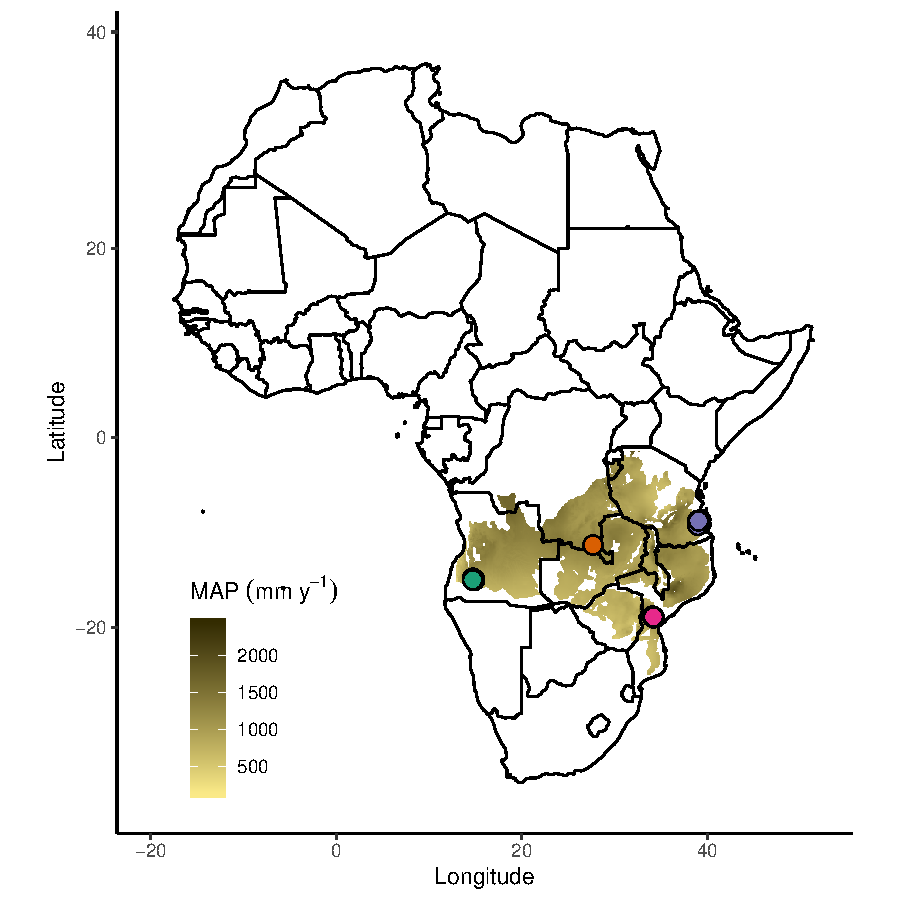
\includegraphics[width=0.475\textwidth]{img/plot_map}}\label{plot_map}}%
    \qquad
\subfloat[]{{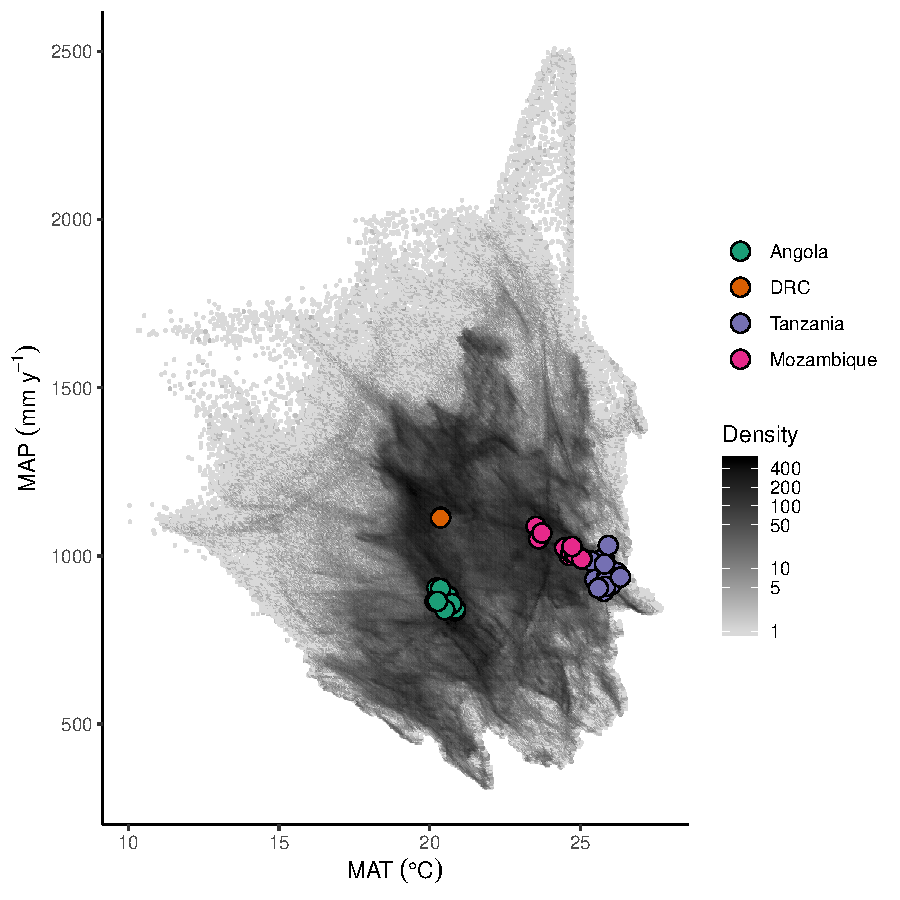
\includegraphics[width=0.475\textwidth]{img/temp_precip}}\label{temp_precip}}%
\caption{Locations of plots used in this study, by~(\textbf{a}) geographic location with respect to the distribution of miombo woodland vegetation (shaded brown according to mean annual precipitation)~\citep{White1983}, and~(\textbf{b})~showing the plot locations compared to the climate space of the miombo ecoregion estimated using the WorldClim dataset over the miombo woodland vegetation extent with a pixel size of 30~arc seconds (0.86 km\textsuperscript{2} at the equator) \citep{Fick2017}. Please note that the density colour scale is log-transformed for visual~clarity.}\label{fig1}
\end{figure}
\unskip


% Table created by stargazer v.5.2.2 by Marek Hlavac, Harvard University. E-mail: hlavac at fas.harvard.edu
% Date and time: Tue, Jan 28, 2020 - 13:54:27
\begin{table}[H] \centering 
  \caption{Description of each group of plots used in the analysis. MAT = Mean Annual Temperature, MAP = Mean Annual Precipitation, CWD = Climatic Water Deficit, DD = Decimal~Degrees.} 
  \label{group_descrip} 
\begin{tabular}{@{\extracolsep{0pt}} rccccccc} 
%\\[-1.8ex]\midrule 
\toprule
% \\[-1.8ex] 
{\textbf{Plot Group}} & \multicolumn{1}{p{1cm}}{\centering \textbf{MAT} \\ \textbf{(\boldmath{$^\circ$}C)}} & \multicolumn{1}{p{1.5cm}}{\centering \textbf{MAP} \\ \textbf{(mm \boldmath{y\textsuperscript{$-$1})}}} & \multicolumn{1}{p{1.5cm}}{\centering \textbf{CWD} \\ \textbf{(mm \boldmath{y\textsuperscript{$-$1})}}} & \multicolumn{1}{p{2cm}}{\centering \textbf{Latitude} \\ \textbf{(DD)}} & \multicolumn{1}{p{2cm}}{\centering \textbf{Longitude} \\ \textbf{(DD)}} & {\textbf{N Plots}} & {\textbf{N Species}} \\
\midrule %\\[-1.8ex] 
Bicuar NP & 20.5 & 864 & $-$815 & $-$15.12 & 14.81 & 15 & 49 \\ 
DRC & 20.4 & 1115 & $-$762 & $-$11.49 & 27.67 & 12 & 89 \\ 
Mozambique & 24.4 & 1029 & $-$662 & $-$18.95 & 34.16 & 15 & 162 \\ 
Tanzania & 25.8 & 956 & $-$754 & $-$9.05 & 39.05 & 22 & 248 \\ \bottomrule

%\midrule \\[-1.8ex] 
\end{tabular} 
\end{table} 


Bicuar National Park covers an area of \textasciitilde{}7900 km\textsuperscript{2}, established as a hunting reserve in 1938, and~later as a national park in 1964 (Figure~\ref{bicuar_map}). While fauna populations in the Park were severely damaged by the Angolan civil war, the~interior of the Park remains as a largely intact mosaic of miombo woodland, Baikiaea-Burkea woodland, shrub/thicket vegetation and seasonally flooded grassland. Encroachment of agriculture and grazing, particularly along the northwest and western boundaries of the Park, has led to a fragmented park boundary with patches of diminished thicket and woodland in areas of previously farmed land that have been protected since park boundaries were re-established following the end of the civil~war.

\rnew{Plots in Tanzania were located predominantly within or near the Mtarure Forest Reserve, administrated by the Tanzania Forest Service and protected from human incursion since their installation. Plots were established between 2010 and 2011 in grassy savanna/woodland areas, with~plots located along the road network with a 1 km buffer from the road. Plots in Mozambique were established in 2004, in~areas of miombo woodland that had been previously used for agriculture but since left fallow, and~areas of undisturbed miombo woodland, located along the road network, with~all plots >250 m from the road. Plots in DRC were established in 2009 and located within a larger 800 ha miombo woodland reserve, which consists of undisturbed miombo woodlands. All plots were located quasi-randomly, with~consideration to accessibility for future woodland censuses.}

\subsection{Plot Data~Collection}

We sampled \nplotsbicuar{} one hectare plots in Bicuar National Park and collated data from a total of \nplots{} one hectare plots across the miombo ecoregion within four sites. Figure~\ref{fig1}a and Table~\ref{group_descrip} show the locations and general description of each site, respectively. Plots in Bicuar were situated at least 500 m from the edge of a woodland patch to prevent edge effects which may have altered tree species~composition.

Within each plot, every tree stem $\ge$5 cm stem diameter was recorded, except~in the DRC plots, where only stems $\ge$10 cm stem diameter were recorded. For~each tree stem the species and stem diameter were recorded. Tree species were identified using local botanists at each site and taxonomy was later checked against the African Plant Database \citep{APD2020}. \rchange{In all sites Palgrave and various other texts were used as a guide for species identification in the field}{At all sites, we used \citet{Palgrave2003}, along with other texts, to~identify tree species}. Specimens that could not be identified in the field, or~subsequently at herbaria, were described as morphospecies. All tree species within the Bicuar National Park plots were identified. Tree coppicing due to fire, herbivory, and~human actions is common in miombo woodlands, therefore, for~trees with multiple stems, each stem $\ge$5 cm stem diameter was recorded, while the parent tree was also recorded for diversity analyses described~below.   

Stem diameter was recorded at 1.3 m from the ground along the stem (diameter at breast height, DBH) as per convention using a diameter tape measure \citep{Kershaw2017}. Where stem abnormalities were present at 1.3 m from the ground, which precluded the accurate estimation of stem diameter at 1.3 m, the~stem diameter was recorded at the nearest 10 cm increment above 1.3 m without significant stem abnormalities \citep{Kershaw2017}. To~ensure consistency among stem diameter values recorded at different heights, when the stem diameter was recorded at a height other than 1.3 m the stem diameter at 1.3 m was estimated from the recorded stem diameter using a cubic polynomial equation which adjusts for tree stem taper. This equation was calibrated on 100 stems measured at multiple heights in Niassa Province, Mozambique (Appendix \ref{appendixa}). Stems below 10 cm stem diameter were not measured in the DRC plots. We therefore estimated the number of 5--10 cm stems in each these plots by extrapolating a linear regression of log stem abundance across the available stem diameter~classes.

In addition to the one hectare plots across the miombo ecoregion, we compared the tree biodiversity of undisturbed areas of miombo woodland in Bicuar National Park with areas of disturbed woodland around the edge of the Park that had been previously farmed via shifting cultivation methods, and~had since been abandoned and reclaimed within the Park boundaries (Figure~\ref{bicuar_map}). We~identified areas previously farmed with the help of park rangers and local residents who identified these areas from memory. We conducted \ndegradplots{} plot surveys of woodland diversity and structure in these areas with 20 \hl{$\times$} %We changed x to multiplication sign, please confirm the same format throughout this article.
50 m (0.1 ha) plots, and~compared their diversity and structure with 20 \hl{$\times$} 50 m subsamples of the \nplotsbicuar{} one hectare plots within the Park interior. Like the one hectare plots, within~these smaller 20 \hl{$\times$} 50 m plots we recorded the species and stem diameter of every tree stem $\ge$5~cm stem~diameter.

\begin{figure}[H]
\centering
	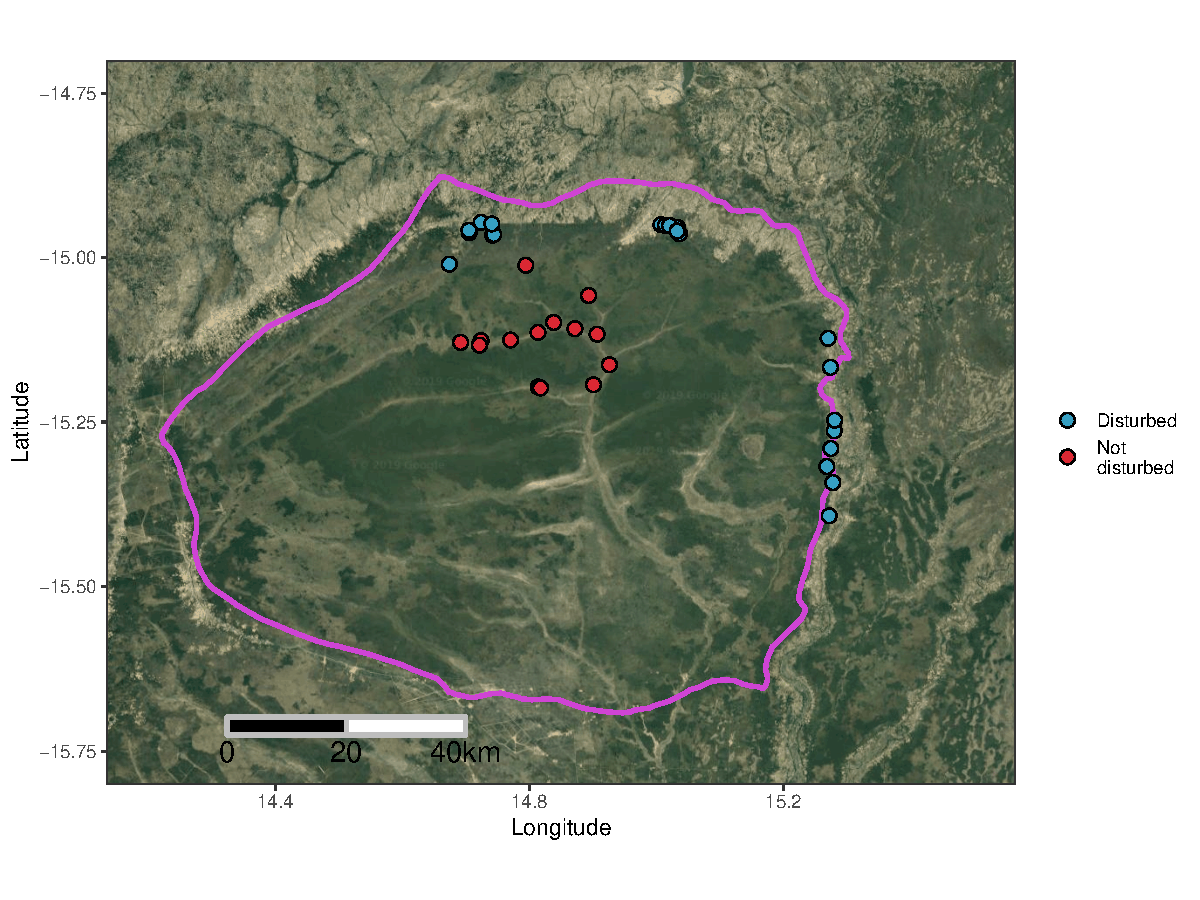
\includegraphics[width=\textwidth]{img/bicuar_map}
	\caption{Location of plots in Bicuar National Park, southwest Angola. The~Park boundary is shown as a pink outline, according to \citet{WDPA2019}. One hectare undisturbed plots are shown as red points, while disturbed 20 $\times$ 50 m (0.1 hectare) plots are shown as blue points. The~map background is a true colour composite satellite image generated using the Google Maps Static Maps API in the \hl{\texttt{ggmap}} %Please confirm the same format of the font throughout this article.
	R package \citep{ggmap}.}
	\label{bicuar_map}
\end{figure}
\unskip

\subsection{Climatic~Data}

The WorldClim dataset \citep{Fick2017} was used to gather data on plot-level climatic conditions. We~estimated Mean Annual Precipitation (MAP) as the mean of total annual precipitation values between 1970 and 2000, and~Mean Annual Temperature (MAT) as the mean of mean annual temperatures between 1970 and 2000. The~seasonality of temperature (MAT SD) was calculated as the standard deviation of monthly temperature per year, respectively. We estimated Climatic Water Deficit (CWD) for each plot according to \citet{Chave2014}, as~the sum of the difference between monthly rainfall and monthly evapotranspiration when the difference is negative, using the dataset available at \url{http://ups-tlse.fr/pantropical_allometry.htm}, which uses data from the WorldClim dataset~1970--2000.

\subsection{Data~Analysis}

We calculated the basal area of each stem ($g_{i}$) using:
\begin{equation}
	g_{i} = \pi{} \times (d_{i} / 2)^{2}
\end{equation}
where $d_{i}$ is the estimated stem diameter of stem $i$ at 1.3 m having accounted for tree taper. We then calculated the total basal area of each plot as the sum of each stem's basal area. For~the DRC plots which lacked 5--10 cm stems, we estimated basal area in this stem diameter class from our extrapolation of stem abundance in the 5--10 cm diameter class, assuming a mean stem diameter of 7.5~cm.

All diversity measures were calculated on individual tree-level data, rather than stem-level data, to~avoid artificial inflation of abundance for those species which readily coppice. We calculated the alpha diversity of each plot using \rnew{both the tree species richness of trees with stems $\ge$5 cm diameter}, and~the Shannon-Wiener index ($H'$) \rnew{(Equation (\ref{shannon}))}, using the \texttt{vegan} package in R \citep{vegan}:

\rnew{
\begin{equation}
	H' = -\sum^{S}_{i=1} p_{i} \ln{p_{i}}
	\label{shannon}
\end{equation}
}
{where $S$ is the total number of species in the plot, $p_{i}$ is the proportional abundance of the $i$th species and $\ln$ is the natural logarithm.}

We calculated the pairwise beta diversity among sites using the S\o{}rensen coefficient ($S_{S}$) \rnew{(Equation~(\ref{sorensen}))} 
\citep{Koleff2003}:

\rnew{
\begin{equation}
	\label{sorensen}
	S_S = \frac{2a}{2a + b + c}
\end{equation}
}
{where $a$ is the number of species shared between two sites, $b$ is the number of species unique to site 1 and $c$ is the number of species unique to site 2. We calculated $S_{S}$ for each pairwise combination of sites using aggregated species composition data from all plots in each site. The~value of $S_{S}$, which ranges between zero and one, was multiplied by 100 to give a ``percentage similarity'' between communities in species composition.}

We estimated abundance evenness for each plot using the Shannon equitability index ($E_{H'}$) \citep{Smith1996} which is the ratio of $H'$ to the log transformed species~richness.

We analysed the difference in alpha diversity measures and woodland structural variables among groups of plots using Analysis of Variance (ANOVA) statistical models, with~a null hypothesis that there was no difference among the mean values of groups of plots. Post-hoc Tukey's HSD tests were used to investigate the degree to which pairwise combinations of plot groups differed in each~case.

We used Non-metric Multidimensional Scaling (NMDS) to assess the variation in species composition among one hectare plots, and~also between disturbed and undisturbed 20 $\times$ 50 m plots within Bicuar National Park, using the \texttt{vegan} R package. The~number of dimensions for NMDS was minimised while ensuring the stress value of the NMDS fit was $\le$0.1. NMDS analyses were run with 500 random restarts to ensure a global solution was reached. We used Bray-Curtis dissimilarity as the optimal measure of ecological distance \citep{Legendre2013}. We fit plot-level estimates of MAP, MAT, the~seasonality of MAT and CWD to the first two axes of the resulting ordination using the \texttt{envfit} function in the \texttt{vegan} R package to investigate how these environmental factors influenced the grouping of species composition among plots. All analyses were conducted in R version 3.6.1 \citep{RCoreTeam2019}.

% Materials and Methods should be described with sufficient details to allow others to replicate and build on published results. Please note that publication of your manuscript implicates that you must make all materials, data, computer code, and protocols associated with the publication available to readers. Please disclose at the submission stage any restrictions on the availability of materials or information. New methods and protocols should be described in detail while well-established methods can be briefly described and appropriately cited.
% Research manuscripts reporting large datasets that are deposited in a publicly available database should specify where the data have been deposited and provide the relevant accession numbers. If the accession numbers have not yet been obtained at the time of submission, please state that they will be provided during review. They must be provided prior to publication.

%%%%%%%%%%%%%%%%%%%%%%%%%%%%%%%%%%%%%%%%%%
\section{Results}
\unskip
\subsection{Alpha~Diversity}

In Bicuar National Park we measured a total of \nbicuartrees{} trees within the one hectare plots, and~across the four sites,  a~total of 25,525 trees were sampled. Trees in Bicuar National Park belonged to \nbicuarspecies{} species within \nbicuarfamilies{} families. Across all four sites we recorded \nspecies{} species from \nfamilies{} families. The~most diverse family within each site and among all plots was Fabaceae with \nfabaceaespecies{} species. We encountered \nbicuaruniquespecies{} tree species in Bicuar National Park which were not found in the other miombo woodland plots (Table \ref{bicuar_species}). The~most common of these unique species were \textit{Brachystegia tamarindoides} (\emph{n} = \nbg{}), \textit{Baikiaea plurijuga} (\emph{n} = \nbp{}) and \textit{Baphia massaiensis} (\emph{n} = \nbm{}). Four species unique to Bicuar National Park within this dataset only had one individual recorded: \textit{Elachyptera parvifolia}, \textit{Entandrophragma spicatum}, \textit{Oldfieldia dactylophylla}, \textit{Peltophorum africanum}.


% Table created by stargazer v.5.2.2 by Marek Hlavac, Harvard University. E-mail: hlavac at fas.harvard.edu
% Date and time: Tue, Jan 28, 2020 - 13:55:01
\begin{table}[H] \centering 
  \caption{Species found in one hectare plots in Bicuar National Park. Stem diameter and basal area are the mean of all stems with the standard error of the mean in parentheses. Number of stems per hectare is the mean of the number of stems in all one hectare plots where stems of that species are present with the standard error of the mean in parentheses. Species found only in Bicuar National Park are marked in bold text with an~asterisk.} 
  \label{bicuar_species} 
\scalebox{.95}[0.95]{\begin{tabular}{@{\extracolsep{-5pt}} rrcccc} \toprule

%\\[-1.8ex]\midrule 
%\midrule \\[-1.8ex] 
{\textbf{Family}} & {\textbf{Species}} & \multicolumn{1}{p{2cm}}{\centering \textbf{Stem Diam.} \\ \textbf{(cm)}} & \multicolumn{1}{p{2cm}}{\centering \textbf{Basal Area} \\ \textbf{(m\textsuperscript{2} ha\boldmath{\textsuperscript{$-$1}})}} & {\textbf{N Stems}} & {\textbf{N Stems \boldmath{ha\textsuperscript{$-$1}}}} \\
\midrule %\\[-1.8ex] 
Fabaceae & Albizia antunesiana & 9.1(2.03) & 0.07(0.040) & 40 & 8(4.81) \\ 
Fabaceae & \textbf{\textasteriskcentered Baikiaea plurijuga} & 28.9(0.75) & 1.72(0.570) & 331 & 55.2(17.83) \\ 
Fabaceae & \textbf{\textasteriskcentered Baphia bequaertii} & 7.4(0.36) & 0.08(0.050) & 127 & 31.8(18.14) \\ 
Fabaceae & \textbf{\textasteriskcentered Baphia massaiensis} & 6.6(0.17) & 0.05(0.020) & 303 & 30.3(11.20) \\ 
Fabaceae & Bobgunnia madagascariensis & 7.8(0.91) & 0.04(0.020) & 32 & 10.7(9.67) \\ 
Fabaceae & \textbf{\textasteriskcentered Brachystegia longifolia} & 12.9(0.48) & 1.14(0.430) & 576 & 115.2(72.67) \\ 
Fabaceae & Brachystegia spiciformis & 11.4(0.52) & 0.74(0.430) & 326 & 81.5(46.56) \\ 
Phyllanthaceae & \textbf{\textasteriskcentered Bridelia mollis} & 5.7(0.31) & 0.02(NA) & 23 & 23(NA) \\ 
Fabaceae & Burkea africana & 8.5(0.33) & 0.39(0.120) & 863 & 71.9(19.11) \\ 
Combretaceae & Combretum apiculatum & 7.6(0.45) & 0.06(0.040) & 60 & 30(15.00) \\ 
Combretaceae & Combretum celastroides & 5.6(0.34) & \textless 0.01(0.000) & 7 & 3.5(2.50) \\ 
Combretaceae & Combretum collinum & 6.3(0.09) & 0.07(0.020) & 609 & 50.8(20.48) \\ 
Combretaceae & \textbf{\textasteriskcentered Combretum hereroense} & 6.7(0.26) & 0.02(0.010) & 73 & 12.2(5.69) \\ 
Combretaceae & \textbf{\textasteriskcentered Combretum psidioides} & 7.4(0.43) & 0.01(0.010) & 33 & 6.6(4.17) \\ 
Combretaceae & Combretum zeyheri & 6.3(0.35) & 0.01(0.000) & 61 & 10.2(3.03) \\ 
Euphorbiaceae & \textbf{\textasteriskcentered Croton gratissimus} & 6.1(1.55) & \textless 0.01(NA) & 4 & 4(NA) \\ 
Ebenaceae & \textbf{\textasteriskcentered Diospyros batocana} & 8.4(2.14) & \textless 0.01(0.000) & 2 & 1(0.00) \\ 
Ebenaceae & \textbf{\textasteriskcentered Diospyros kirkii} & 9.3(1.64) & 0.03(NA) & 11 & 11(NA) \\ 
Apocynaceae & Diplorhynchus condylocarpon & 8.2(0.52) & 0.08(0.060) & 174 & 19.3(7.57) \\ 
Malvaceae & \textbf{\textasteriskcentered Dombeya rotundifolia} & 5.5(0.19) & \textless 0.01(NA) & 2 & 2(NA) \\ 
Celastraceae & \textbf{\textasteriskcentered Elachyptera parvifolia} & 7.3(NA) & \textless 0.01(NA) & 1 & 1(NA) \\ 
Meliaceae & \textbf{\textasteriskcentered Entandrophragma spicatum} & 14.6(NA) & \textless 0.01(NA) & 1 & 1(NA) \\ 
Fabaceae & Erythrophleum africanum & 9.0(0.84) & 0.10(0.040) & 128 & 18.3(6.82) \\ 
Rubiaceae & \textbf{\textasteriskcentered Gardenia volkensii} & 5.6(1.15) & \textless 0.01(0.000) & 5 & 2.5(1.50) \\ 
Fabaceae & \textbf{\textasteriskcentered Guibourtia coleosperma} & 7.2(1.00) & 0.02(0.010) & 31 & 6.2(3.54) \\ 
Phyllanthaceae & Hymenocardia acida & 5.9(1.25) & \textless 0.01(NA) & 6 & 6(NA) \\ 
Fabaceae & Julbernardia paniculata & 10.1(0.21) & 0.92(0.200) & 1624 & 162.4(50.60) \\ 
Fabaceae & \textbf{\textasteriskcentered Lonchocarpus nelsii} & 13.4(0.88) & 0.15(0.030) & 165 & 15(2.77) \\ 
Dipterocarpaceae & \textbf{\textasteriskcentered Monotes angolensis} & 7.4(0.83) & \textless 0.01(0.000) & 2 & 1(0.00) \\ 
Ochnaceae & \textbf{\textasteriskcentered Ochna pulchra} & 6.5(0.80) & 0.01(0.000) & 26 & 8.7(3.76) \\ 
Picrodendraceae & \textbf{\textasteriskcentered Oldfieldia dactylophylla} & 8.5(NA) & \textless 0.01(NA) & 1 & 1(NA) \\ 
Fabaceae & \textbf{\textasteriskcentered Peltophorum africanum} & 11.5(NA) & \textless 0.01(NA) & 1 & 1(NA) \\ 
Fabaceae & Pericopsis angolensis & 8.4(0.61) & 0.06(0.020) & 97 & 12.1(5.08) \\ 
Phyllanthaceae & Pseudolachnostylis maprouneifolia & 6.7(0.45) & 0.03(0.010) & 84 & 9.3(3.00) \\ 
Combretaceae & \textbf{\textasteriskcentered Pteleopsis anisoptera} & 6.8(0.46) & 0.07(0.020) & 81 & 20.2(15.11) \\ 
Fabaceae & Pterocarpus angolensis & 13.0(0.61) & 0.15(0.100) & 102 & 17(8.65) \\ 
Fabaceae & \textbf{\textasteriskcentered Pterocarpus lucens} & 6.9(0.94) & \textless 0.01(NA) & 4 & 4(NA) \\ 
Rubiaceae & \textbf{\textasteriskcentered Rothmannia engleriana} & 6.8(0.66) & \textless 0.01(0.000) & 5 & 1.7(0.67) \\ 
Euphorbiaceae & \textbf{\textasteriskcentered Schinziophyton rautanenii} & 8.0(2.82) & \textless 0.01(NA) & 3 & 3(NA) \\ 
Polygalaceae & Securidaca longepedunculata & 7.3(1.12) & \textless 0.01(0.010) & 4 & 2(1.00) \\ 
Loganiaceae & Strychnos cocculoides & 10.4(1.17) & 0.03(0.020) & 19 & 6.3(3.53) \\ 
Loganiaceae & \textbf{\textasteriskcentered Strychnos pungens} & 6.1(0.48) & \textless 0.01(0.000) & 18 & 3.6(0.93) \\ 
Loganiaceae & Strychnos spinosa & 6.8(0.36) & 0.02(0.010) & 97 & 9.7(4.07) \\ 
Combretaceae & \textbf{\textasteriskcentered Terminalia brachystemma} & 6.5(0.21) & 0.04(0.020) & 174 & 29(12.04) \\ 
Combretaceae & Terminalia sericea & 7.1(0.28) & 0.06(0.030) & 214 & 23.8(12.18) \\ 
Ximeniaceae & Ximenia americana & 6.1(0.53) & \textless 0.01(0.000) & 7 & 1.8(0.25) \\ 
Sapindaceae & Zanha africana & 9.4(1.12) & 0.01(NA) & 6 & 6(NA) \\ 
Rhamnaceae & \textbf{\textasteriskcentered Ziziphus abyssinica} & 5.9(1.13) & \textless 0.01(NA) & 2 & 2(NA) \\ \bottomrule

%\midrule \\[-1.8ex] 
\end{tabular}}
\end{table} 


Alpha diversity in Bicuar National Park was low compared to other sites (Figure~\ref{div_box}). Mean~$H'$ across plots in Bicuar National Park was \bicuarshannon{}. An~ANOVA showed a significant difference in $H'$ among sites (\lmshannon{}, Table~\ref{anova_table}), and~a post-hoc Tukey's test showed that $H'$ in plots in Bicuar National Park was significantly different from those in DRC ($H'$ = \drcshannon{}, \tukeyshannonbicuardrc{}), Mozambique ($H'$ = \nhamshannon{}, \tukeyshannonbicuarnham{}) and Tanzania ($H'$ = \kilwashannon{}, \tukeyshannonbicuarkilwa{}). Variation in $H'$ is large within Bicuar National Park, with~$H'$ ranging from \bicuarminshannon{} to \bicuarmaxshannon{}, but~this was a similar range to other sites. In~contrast, the~range of species richness within Bicuar National Park was much lower than other sites, suggesting that the wide range in $H'$ was caused by variation in abundance~evenness.

\begin{figure}[H]
\centering
	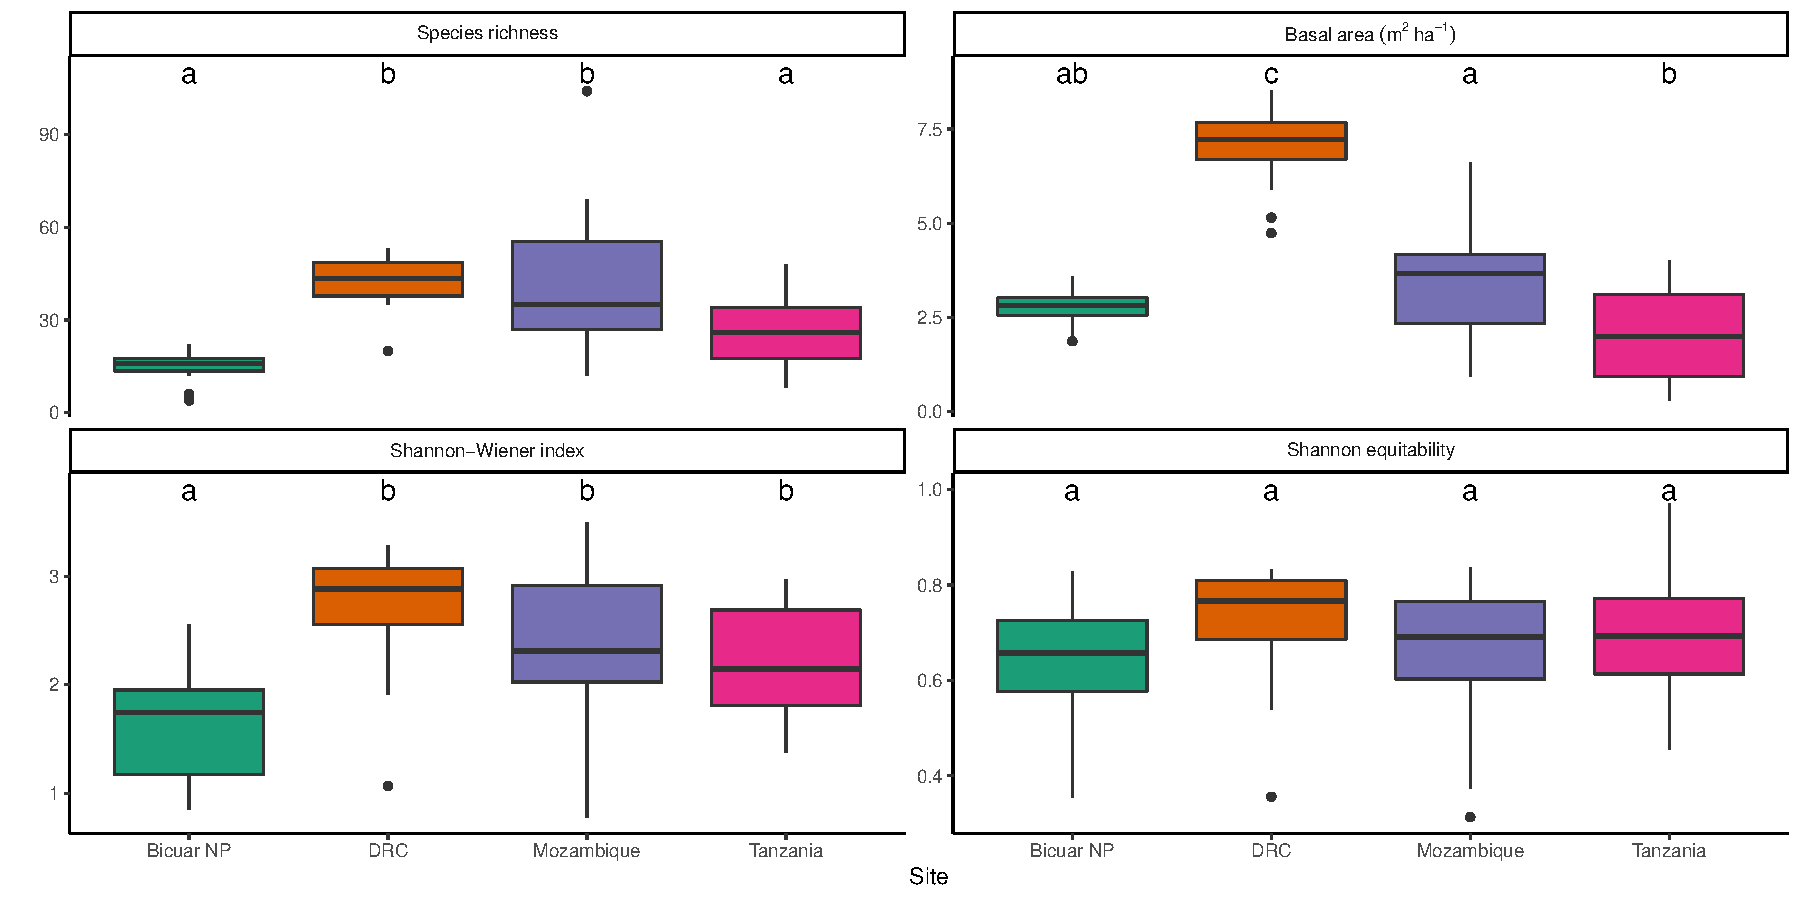
\includegraphics[width=\textwidth]{img/div_box}
	\caption{Variation of alpha diversity estimates and basal area among sites. Boxes bound the 1st and 3rd quartiles, with~the median within the box. Whiskers represent 1.5 times the interquartile range plus or minus the 1st and 3rd quartiles, respectively. Values found beyond the whiskers are shown individually as points. \rnew{Letter labels above each box refer to groupings from post-hoc Tukey's tests on the ANOVA of each diversity/structure variable. Sites sharing a letter do not differ significantly (\mbox{\emph{p} < 0.05})}.}
    \label{div_box}
\end{figure}
\unskip


% Table created by stargazer v.5.2.2 by Marek Hlavac, Harvard University. E-mail: hlavac at fas.harvard.edu
% Date and time: Fri, Mar 27, 2020 - 14:32:56
\begin{table}[H] \centering 
  \caption{Results of ANOVA tests for alpha diversity metrics and plot basal area, among~the four sites. Mean values for each site with standard errors in parentheses are shown. Asterisks indicate the \emph{p}-value of individual sites in each ANOVA (*** <0.001, ** <0.01, * <0.05, \hl{.} <0.1).}  %We can't find ``.'' in table body, please add them or remove the explanation.
  \label{anova_table} 
\begin{tabular}{@{\extracolsep{0pt}}lcccc} \toprule

%\\[-1.8ex]\midrule 
%\midrule \\[-1.8ex] 
 & \multicolumn{4}{c}{\hl{\textbf{Dependent Variable:}}} \\  %Is italic necessary?
\cmidrule{2-5} 
%\\[-1.8ex]
 & \textbf{Species Richness} & \textbf{Basal Area} & \textbf{Shannon \boldmath{($H'$)}} & \textbf{Shannon Equit. \boldmath{($E_{H}$)}} \\ 
%\\[-1.8ex] 
& \textbf{(1)} & \textbf{(2)} & \textbf{(3)} & \textbf{(4)}\\ \midrule

 DRC & 27.920 *** & 4.175  *** & 1.055  *** & 0.080 \\ 
  & (5.538) & (0.452) & (0.236) & (0.053) \\ 
%  & & & & \\ 
 Tanzania & 12.440 ** & $-$0.721 * & 0.605 *** & 0.064 \\ 
  & (4.788) & (0.391) & (0.204) & (0.046) \\ 
 % & & & & \\ 
 Mozambique & 27.930 *** & 0.653 & 0.792 *** & 0.028 \\ 
  & (5.221) & (0.427) & (0.223) & (0.050) \\ 
%  & & & & \\ 
 Constant & 14.330 *** & 2.778 *** & 1.617 *** & 0.631 *** \\ 
  & (3.692) & (0.302) & (0.158) & (0.035) \\ 
  %& & & & \\ 
\midrule %\\[-1.8ex] 
Observations & 64 & 64 & 64 & 64 \\ 
Adjusted R$^{2}$ & 0.363 & 0.691 & 0.237 & 0.003 \\ 
Residual Std. Error (df = 60) & 14.300 & 1.168 & 0.611 & 0.137 \\ 
F Statistic (df = 3; 60) & 12.980 *** & 48.040 *** & 7.537 *** & 1.000 \\ \bottomrule

%\midrule 
%\midrule \\[-1.8ex] 
\end{tabular} 
\end{table}
\unskip 


\subsection{Beta~Diversity}

The NMDS of plot species composition among one hectare plots was run with four dimensions. The~stress value was \nmdsstress{}. Plot diversity in Bicuar National Park formed three distinct groups within axes 1 and 2 of the NMDS ordination. Bicuar plots 9, 13 and~15 were characterised by high abundances of \textit{Baikiaea plurijuga}, \textit{Baphia massaiensis} and \textit{Croton gratissimus}, according to species scores from the NMDS. Bicuar plots 4, 11 and~12 were characterised  by \textit{Brachystegia tamarindoides} and~\textit{Ochna pulchra}. The~third group consisting of the remaining seven plots surprisingly had a species composition most similar to that of plots in the DRC group according to the NMDS, sharing the core miombo species of \textit{Julbernardia paniculata} and \textit{Pterocarpus angolensis}. This group of plots in Bicuar National Park was further characterised by the abundance of \textit{Pterocarpus lucens}, \textit{Strychnos pungens} and \textit{Bridelia mollis} however, which were not present in the DRC plots. All environmental factors fitted to the NMDS ordination correlated significantly with the grouping of plots (Figure~\ref{fig4}a). MAT explained the most variation in plot position on the first two \hl{NMDS axes} %Please check throughout this article if R should be italicized.
(\nmdsmat{}), followed by CWD (\nmdsmapsd{}), the~seasonality of MAT (\nmdsmatsd{}) and MAP (\nmdsmap{}). Variation in MAP explained much of the difference among plots in Bicuar National Park versus those in Tanzania and Mozambique. Axes 3 and 4 showed a greater degree of overlap in species composition among plot groups, with~plots from Bicuar National Park similar to a select few plots in both Tanzania and Mozambique (Figure~\ref{fig4}b). Axis 3 distinguished plots in Bicuar NP from those in DRC, while plots from all geographic area overlapped in their distribution across Axis 4. Axes 3 and 4 largely reflected distribution patterns of less abundant species and not the dominant species in the~vegetation.


\begin{figure}[H]
	\centering
	\subfloat[]{{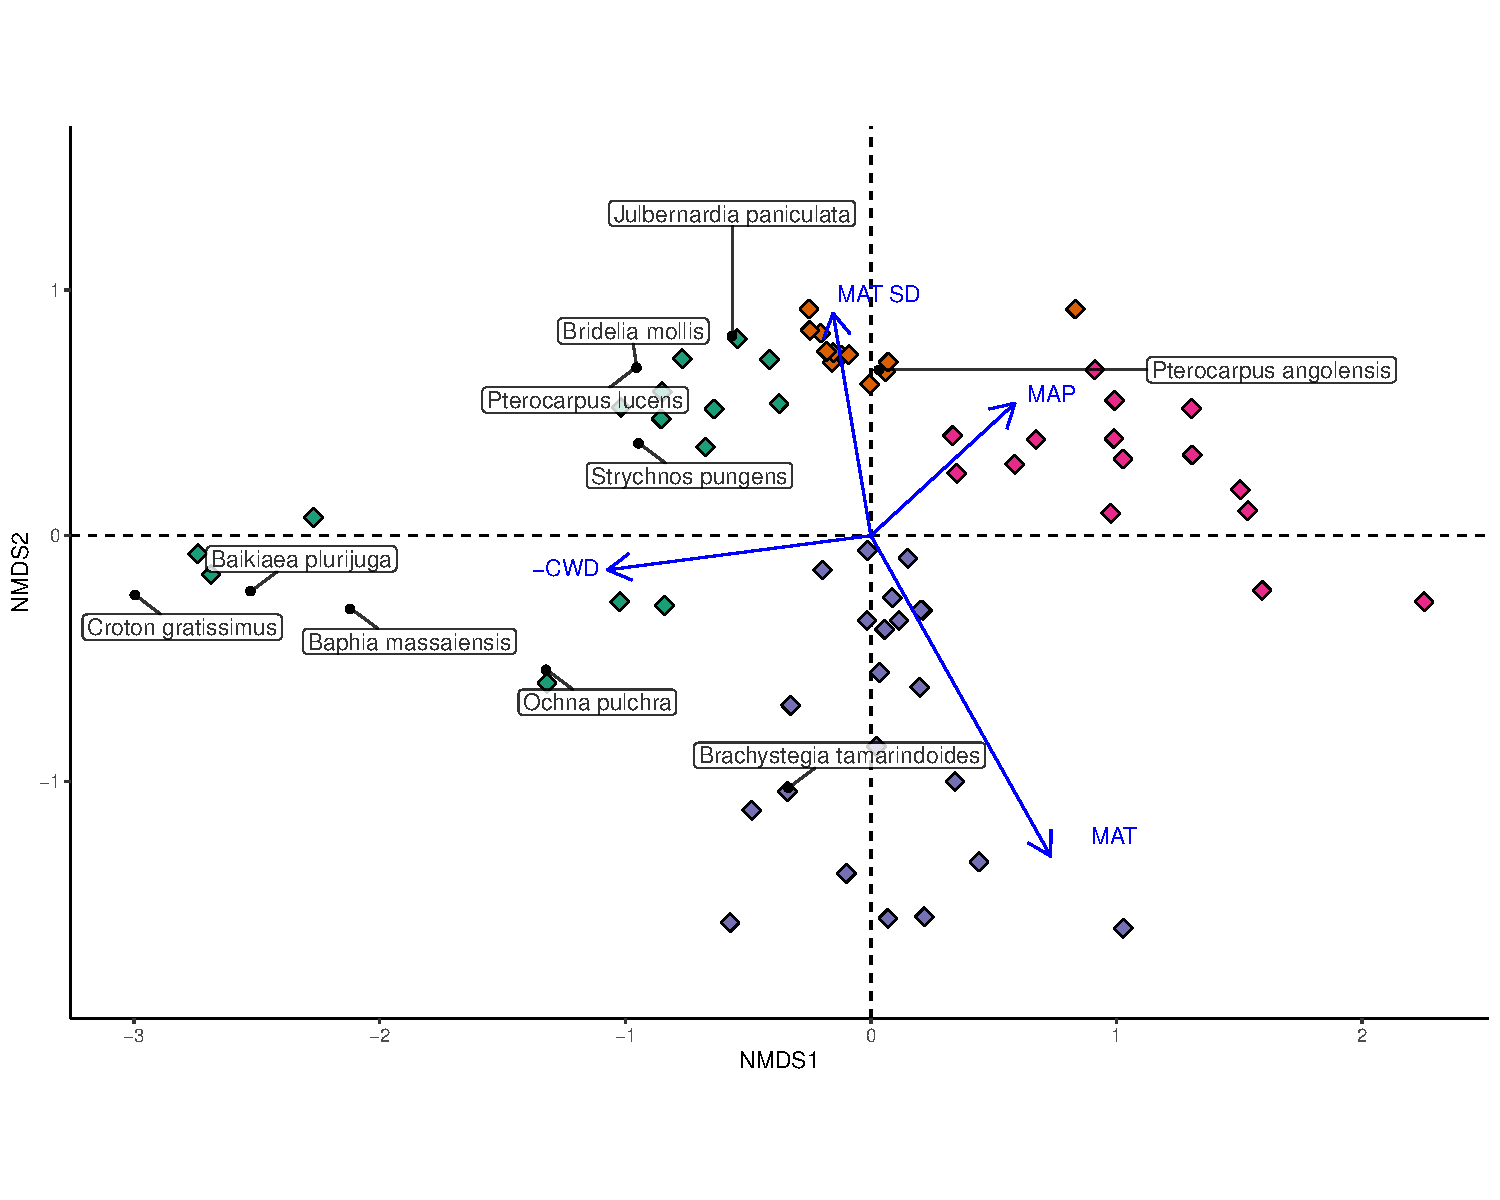
\includegraphics[width=0.475\textwidth]{img/all_nmds_envfit}}\label{all_nmds_envfit}}%
    \qquad
\subfloat[]{{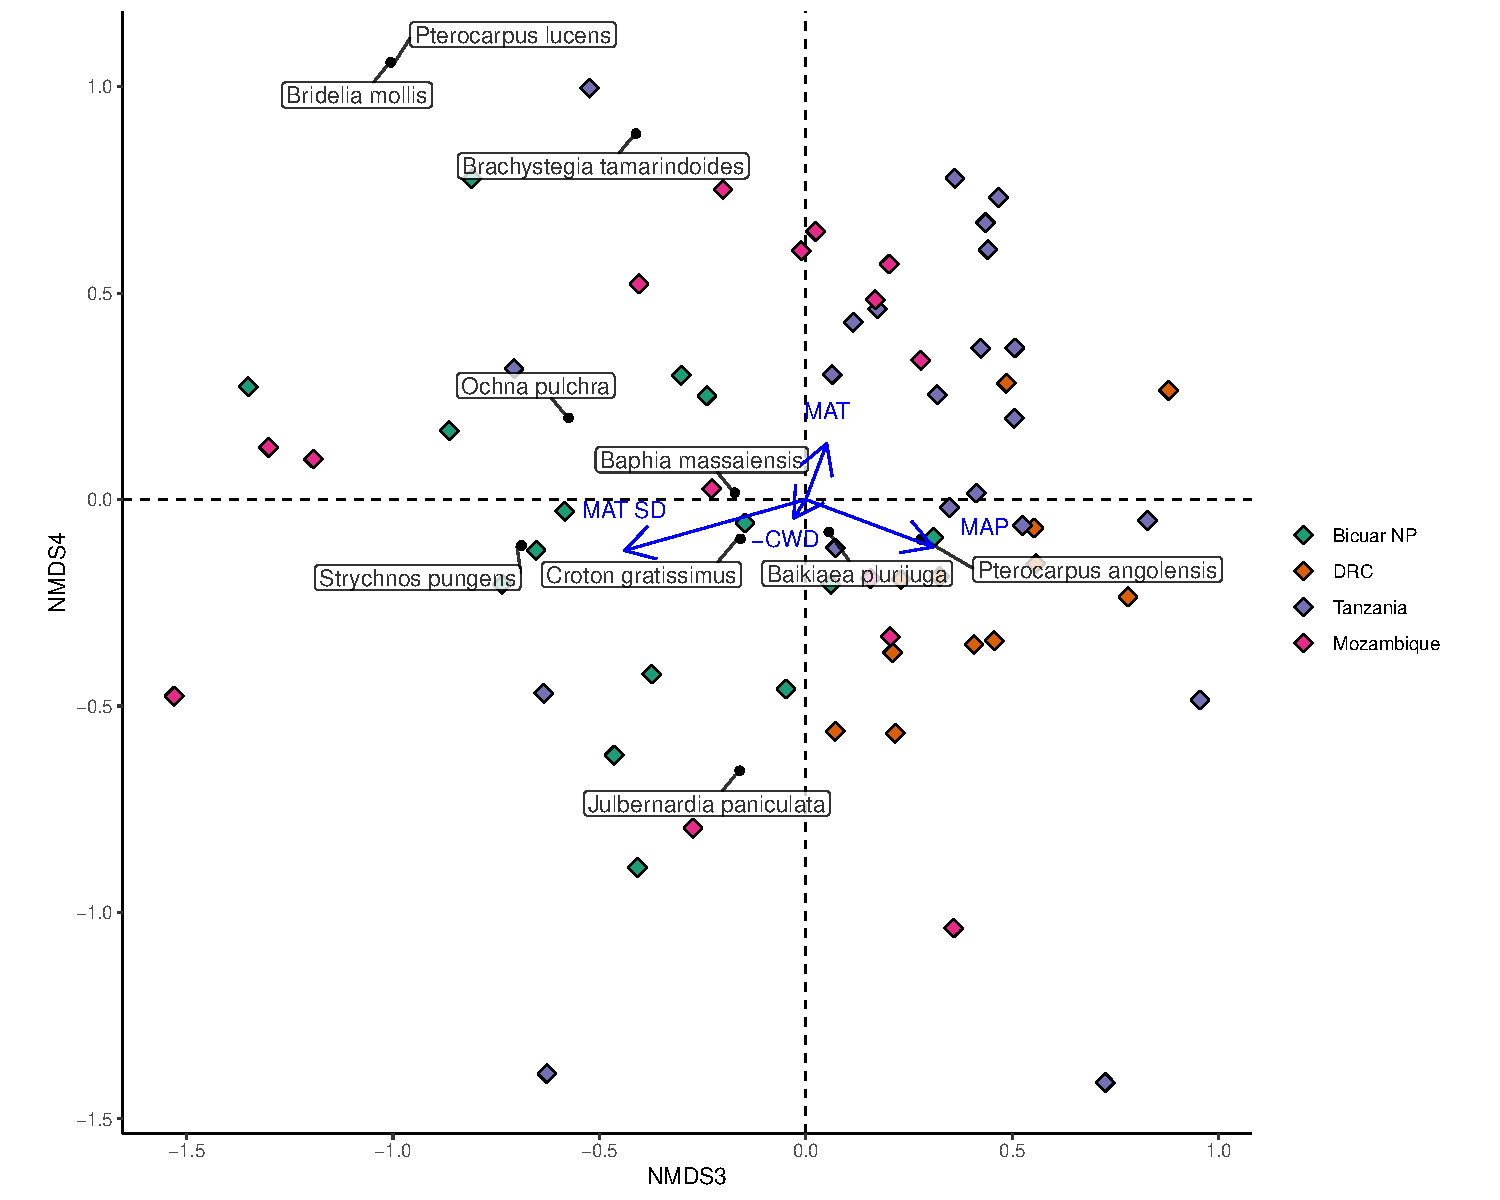
\includegraphics[width=0.475\textwidth]{img/all_nmds_envfit_low}}\label{all_nmds_envfit_low}}%
\caption{Environmental factors fitted to axes 1 and 2 (\textbf{a}), 3 and 4 (\textbf{b}) of the NMDS ordination of species composition of one hectare plots, showing the variation in plot species composition within and among sites. Diamonds are plot scores coloured by site. The~lengths of arrows indicating environmental factor fits are scaled by R\textsuperscript{2}. Arrows point in the direction of increasing values of that environmental factor. Please note that Climatic Water Deficit (CWD) is expressed more intuitively as the negative inverse of CWD, thus larger values indicate higher levels of~CWD.}\label{fig4}
\end{figure}

The pairwise S\o{}rensen coefficient of percentage similarity ($S_{S}$) showed that the species composition of plots in Bicuar National Park had low similarity with other sites in the study, sharing a few species with other sites (Table \ref{site_pairs_js}). Similar to the NMDS, these results show that plots in Bicuar National Park are most similar to those found in~DRC. 


% Table created by stargazer v.5.2.2 by Marek Hlavac, Harvard University. E-mail: hlavac at fas.harvard.edu
% Date and time: Tue, Jan 28, 2020 - 14:16:40
\begin{table}[H] \centering 
  \caption{Pairwise beta diversity comparison of plot groups measured by the S\o{}rensen coefficient ($S_s$) of percentage similarity of aggregated plot level data from each of the four sites. Values in parentheses are the number of species unique to each site in each~comparison.} 
  \label{site_pairs_js} 
\begin{tabular}{@{\extracolsep{0pt}} rrcc} \toprule

%\\[-1.8ex]\midrule 
%\midrule \\[-1.8ex] 
\textbf{Site 1} & \textbf{Site 2} & \boldmath{$S_{S}$} & \textbf{Shared Species} \\
\midrule% \\[-1.8ex] 
Bicuar \hl{NP (34)} %Please check if there should be a space before the (.
& \hl{DRC (74)} & 20.6 & $14$ \\ 
Bicuar \hl{NP (34)} & Tanzania (147) & 13.4 & $14$ \\ 
Bicuar NP (37) & Mozambique (236) & 7.5 & $11$ \\ 
DRC (64) & Tanzania (137) & 19.3 & $24$ \\ 
DRC (69) & Mozambique (228) & 11.3 & $19$ \\ 
Tanzania (139) & Mozambique (225) & 10.8 & $22$ \\ \bottomrule

%\midrule \\[-1.8ex] 
\end{tabular} 
\end{table}
\unskip 


\subsection{Woodland~Structure}

Mean basal area of plots in Bicuar National Park was \babicuar{} m\textsuperscript{2} ha\textsuperscript{$-$1}, ranging from \bicuarbamin{} to \bicuarbamax{} m\textsuperscript{2} ha\textsuperscript{$-$1} (Figure~\ref{div_box}). An~ANOVA showed a significant difference in basal area among sites (\lmba{}), and~a post-hoc Tukey's test showed that basal area in Bicuar National Park was significantly lower than plots in DRC (BA = \badrc{} m\textsuperscript{2} ha\textsuperscript{$-$1}, \tukeybabicuardrc{}), but~there were no significant differences between Bicuar and Mozambique (BA = \banham{} m\textsuperscript{2} ha\textsuperscript{$-$1}, \tukeybabicuarnham{}) or Tanzania (BA = \bakilwa{} m\textsuperscript{2} ha\textsuperscript{$-$1}, \tukeybabicuarkilwa{}) (Figure~\ref{div_box}). Additionally, Bicuar plots had less variation in basal area among plots than other sites. Plots in Bicuar with the highest basal area were dominated by \textit{Baikiaea plurijuga} and \textit{Baphia massaiensis} (Plots 9, 13, and~15). 

The stem diameter abundance distribution in Bicuar National Park was comparable with other sites (Figure~\ref{stem_ab_dbh_bin}), albeit with fewer stems in each class. The~slope of log mean stem size distribution among diameter bins was \dbhslopebicuar{} in Bicuar National Park, \dbhslopedrc{} in DRC, \dbhslopekilwa{} in Tanzania, and~\dbhslopenham{} in~Mozambique.  

\begin{figure}[H]
\centering
	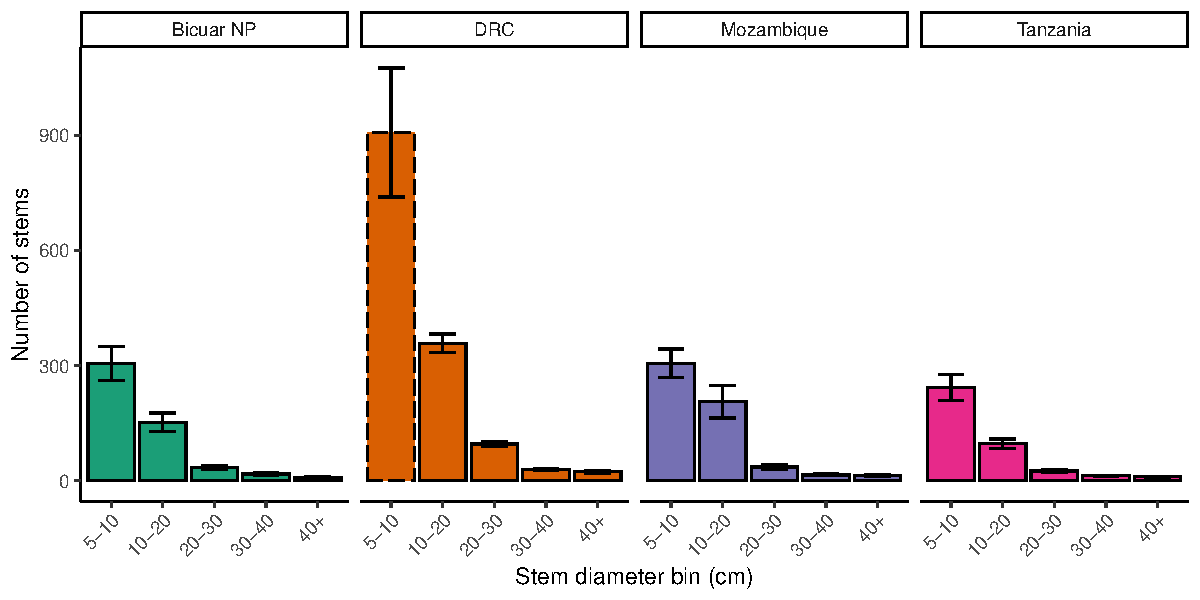
\includegraphics[width=\textwidth]{img/stem_ab_dbh_bin_group}
	\caption{Ranked variation between plots in stem number within each site, with~bars according to stem diameter class. Error bars are the mean $\pm$ 1 standard error. The~dashed bar for the DRC 5--10 cm stem diameter class indicates that these measurements were estimated by extrapolating a linear regression of log stem abundance across the available stem diameter classes for~DRC.}
	\label{stem_ab_dbh_bin}
\end{figure}
\unskip

\subsection{Effect of Disturbance via Shifting Cultivation on Diversity within Bicuar National~Park}

There was a clear difference in the species composition of previously farmed disturbed woodland plots and undisturbed woodland plots, but~with some overlap (Figure~\ref{bicuar_degrad_nmds}). Notably, Plots 4 and 7 in putatively undisturbed woodland have a species composition more resembling the disturbed plots. These two plots were dominated by \textit{Brachystegia tamarindoides} and \textit{Burkea africana}, with~\textit{B. africana} being a species which occurred frequently as a pioneer in the disturbed plots. The~undisturbed plots 15, 13 and~9 represent distinct outliers in the NMDS. These three plots were dominated by \textit{Baikiaea plurijuga} which was not encountered in the disturbed plots. The~most common species in the disturbed plots was \textit{Baphia massaiensis} (\emph{n} = \nbmdegrad{}), with~a mean stem diameter of \bmdbhdegrad{} cm, while in the undisturbed plots the most common species was \textit{Julbernardia paniculata} (\emph{n} = \njpdegrad{}), with~a mean stem diameter of \jpdbhbicuar{} cm. Mean alpha diversity was marginally higher in disturbed plots ($H'$ = \degradshannon{}) than in undisturbed plots ($H'$ = \bicuarsubshannon{}) and an ANOVA showed that there was a significant difference in $H'$ between the two plot types (\lmshannondegrad{}) (Figure~\ref{degrad_box}, Table~\ref{degrad_anova_table}). Mean plot species richness was also lower in undisturbed plots (\bicuarsubrich{}) than disturbed plots (\degradrich{}). Mean $E_{H'}$ was \degradequit{} in disturbed plots and \bicuarsubequit{} in undisturbed plots but there was no significant difference between disturbed and undisturbed plots according to an ANOVA (\lmequitdegrad{}). \ndegradonlyspecies{} species were found only in the disturbed plots and not in the undisturbed plots. The~most common of these were \textit{Combretum celastroides} (\emph{n} = \nccdegrad{}), \textit{Acacia reficiens} (\emph{n} = \nvrdegrad{}), and~\textit{Gardenia ternifolia} (\emph{n} = \ngtdegrad{}). \nbigonlyspecies{} were found only in undisturbed plots, the~most common being \textit{Brachystegia spiciformis} (\emph{n} = \nbsbig{}), \textit{Baikiaea plurijuga} (\mbox{\emph{n} = \nbpbig{}}) and \textit{Combretum apiculatum} (\emph{n} = \ncabig{}). Mean basal area was higher in undisturbed plots (\bicuarsubba{}~m\textsuperscript{2}~ha\textsuperscript{$-$1}) than disturbed plots (\degradba{} m\textsuperscript{2} ha\textsuperscript{$-$1}). 

Mean stem density was higher in disturbed plots (\stemdensdegrad{} stems ha\textsuperscript{$-$1}) than undisturbed plots (\stemdensbicuar{} stems ha\textsuperscript{$-$1}). The~stem diameter abundance distribution in disturbed plots showed that many more stems were from the 5--10 cm diameter class in disturbed plots, while the disturbed plots had fewer stems in the 10--20 cm size class. Both disturbed and undisturbed plots had a similar abundance of stems in larger stem diameter classes (Figure~\ref{degrad_dbh_bin}). Multi-stemmed trees in disturbed plots tended to have a greater number of stems per tree (\multistemdegrad{}) than multi-stemmed trees in undisturbed plots (\multistembicuar{}).

\begin{figure}[H]
\centering
	\includegraphics[width=0.75\textwidth]{img/bicuar_degrad_nmds}
	\caption{NMDS ordination of species composition of \mbox{20 $\times$ 50 m} (0.1 ha) plots showing plot scores as coloured diamonds located in disturbed (blue) and undisturbed (red) areas of woodland in Bicuar National~Park.}
	\label{bicuar_degrad_nmds}
\end{figure}
\unskip

\begin{figure}[H]
\centering
	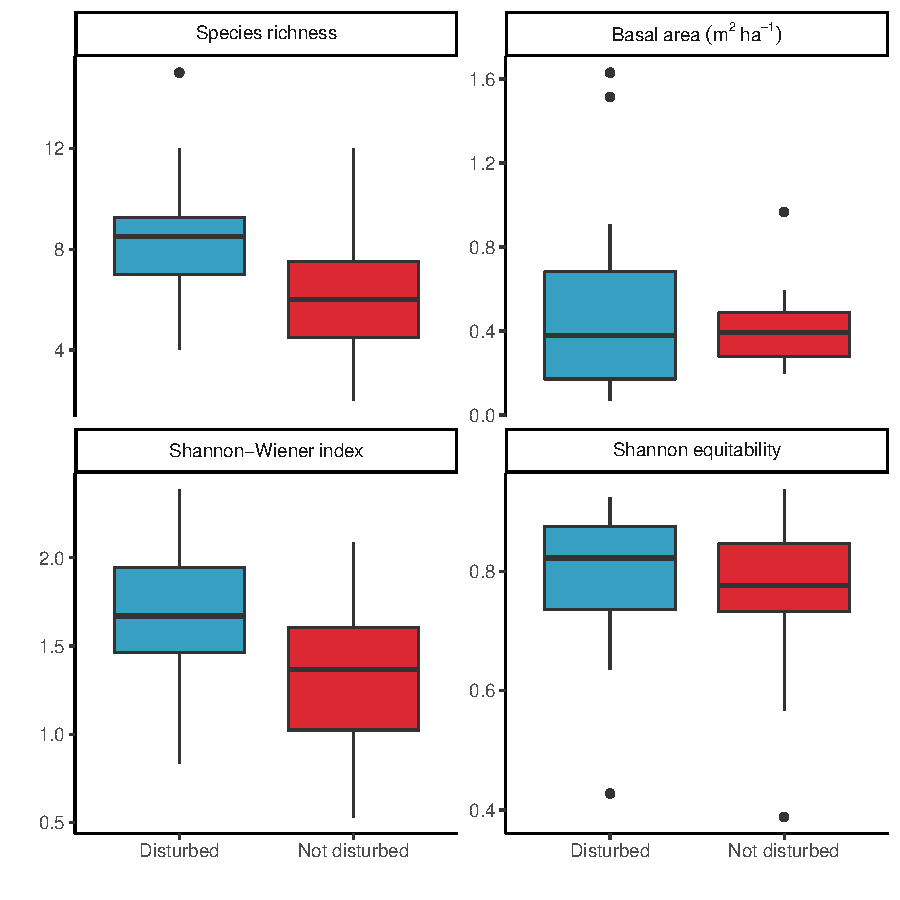
\includegraphics[width=0.8\textwidth]{img/degrad_box}
	\caption{The variation in diversity and woodland structure between disturbed and undisturbed \mbox{20 $\times$ 50 m} (0.1 ha) plots in Bicuar National Park. Boxes bound the 1st and 3rd quartiles, with~the median within the box. Whiskers represent 1.5 times the interquartile range plus or minus the 1st and 3rd quartiles, respectively. Values found beyond the whiskers are shown individually as~points.}
	\label{degrad_box}
\end{figure}
\unskip


% Table created by stargazer v.5.2.2 by Marek Hlavac, Harvard University. E-mail: hlavac at fas.harvard.edu
% Date and time: Fri, Mar 27, 2020 - 14:54:58
\begin{table}[H] \centering 
  \caption{Results of ANOVA tests for alpha diversity metrics and plot basal area, between~disturbed and undisturbed plots in Bicuar National Park. Mean values for each group of plots with standard errors in parentheses are shown. Asterisks indicate the \emph{p}-value of individual sites in each ANOVA (*** <0.001, ** <0.01, \mbox{* <0.05}, \hl{.} <0.1).} %We can't find * and . in table body, please add them or remove explanation.
  \label{degrad_anova_table} 
\begin{tabular}{@{\extracolsep{0pt}}lcccc} \toprule

%\\[-1.8ex]\midrule 
%\midrule \\[-1.8ex] 
 & \multicolumn{4}{c}{\textit{\textbf{Dependent Variable:}}} \\ %Is italic necessary?
\cmidrule{2-5} 
%\\[-1.8ex]
 & \textbf{Species Richness} & \textbf{Basal Area} & \textbf{Shannon (\boldmath{$H'$})} & \textbf{Shannon Equit. (\boldmath{$E_{H}$})} \\ 
\midrule %\\[-1.8ex] 
 Disturbed & 2.450 *** & 0.098 & 0.372 ** & 0.035 \\ 
  & (0.859) & (0.122) & (0.140) & (0.045) \\ 
%  & & & & \\ 
 Constant & 6.200 *** & 0.416 *** & 1.311 *** & 0.756 *** \\ 
  & (0.650) & (0.092) & (0.106) & (0.034) \\ 
 % & & & & \\ 
\midrule %\\[-1.8ex] 
Observations & 35 & 35 & 35 & 35 \\ 
R$^{2}$ & 0.198 & 0.019 & 0.176 & 0.018 \\ 
Residual Std. Error (df = 33) & 2.516 & 0.357 & 0.410 & 0.131 \\ 
F Statistic (df = 1; 33) & 8.126 *** & 0.639 & 7.040 ** & 0.617 \\ \bottomrule

%\midrule 
%\midrule \\[-1.8ex] 
\end{tabular} 
\end{table}
\unskip 


\begin{figure}[H]
\centering
	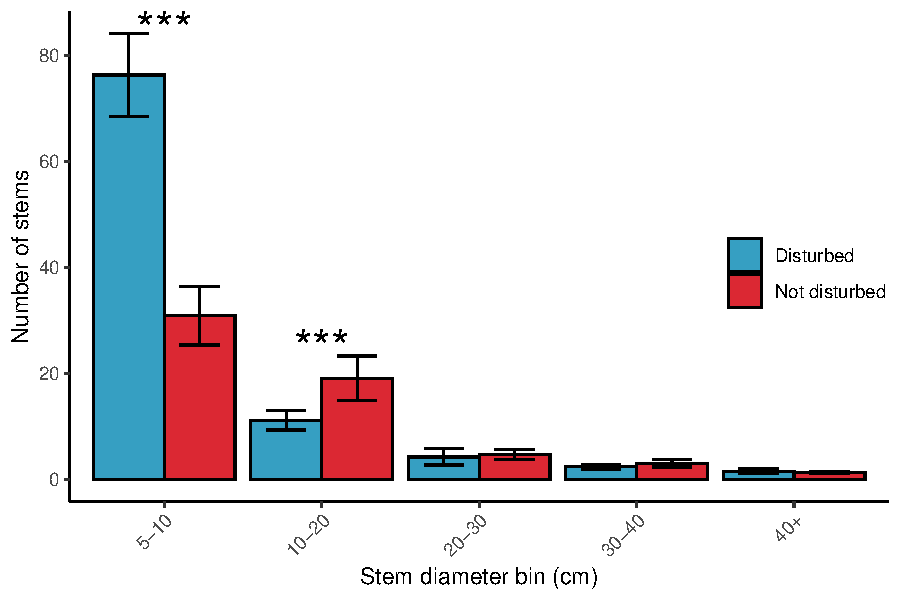
\includegraphics[width=0.8\textwidth]{img/degrad_dbh_bin}
	\caption{Ranked variation between disturbed and undisturbed plots in stem number, with~bars according to stem diameter class. Error bars are the mean $\pm$ 1 standard error. Asterisks above pairs of bars refer to the \emph{p}-values of Poisson general linear models which tested whether disturbed and undisturbed plots differ in the number of stems for different stem diameter classes (*** <0.001, ** <0.01, * <0.05, . <0.1).} %We can't find *,   ** and . in figure body, please add them or remove explanation.
	\label{degrad_dbh_bin}
\end{figure}

%% If the documentclass option "submit" is chosen, please insert a blank line before and after any math environment (equation and eqnarray environments). This ensures correct linenumbering. The blank line should be removed when the documentclass option is changed to "accept" because the text following an equation should not be a new paragraph. 

%%%%%%%%%%%%%%%%%%%%%%%%%%%%%%%%%%%%%%%%%%
\section{Discussion}
\unskip
\subsection{Comparison of Bicuar National Park with Other Woodlands across the Miombo~Ecoregion}

We compared the tree species diversity and woodland structure of arid woodlands in Bicuar National Park in southwest Angola with three other woodland sites across the miombo ecoregion. Our~results show that Bicuar National Park is distinct in both woodland structure and species composition from these other woodlands. Notably, plots in Bicuar National Park contained 27 tree species which did not occur at other sites. This lends support for the Hu\'{i}la Plateau as an important area for conservation of southern African woodland landscapes. The~woodlands in Bicuar National Park were of low tree basal area, with~few large trees except in plots dominated by \textit{Baikiaea plurijuga}. Many~other studies have drawn a relationship between water availability and basal area \citep{Terra2018, Strickland2016}, and~our study supports this, with~Bicuar National Park being the most arid of the four sites considered in our study. The~NMDS of species composition also suggests that plots in Bicuar National Park are influenced by aridity. While there are more arid woodlands within southern Africa, with~Mopane woodlands for example often being particularly dry, these plots in Bicuar National park represent particularly dry miombo~woodlands.

\subsection{Delineation of Woodland Types within Bicuar National~Park}

Within Bicuar National Park, three distinct woodland types were identified. The~first, dominated by \textit{Baikiaea plurijuga} and \textit{Baphia massaiensis} represents the Baikiaea woodland type commonly found to the south of the miombo ecoregion \citep{Timberlake2010}. This is supported by \citet{Chisingui2018} who also found Baikiaea woodlands as a distinct woodland type in the Park. \textit{B. plurijuga} has been identified as an important species for conservation, being attractive for selective logging due to its large \mbox{stature~\citep{Ngandwe2017, Wallenfang2015}}. The~woodlands created by \textit{B. plurijuga} are also an important habitat for elephants (\textit{Loxodonta africana})~\citep{Sianga2017, Mukwashi2012}, with~Bicuar National Park and Mupa National Park being key refugia for this animal in the Hu\'{i}la plateau region. The~second woodland type, dominated by \textit{Brachystegia tamarindoides} and \textit{Ochna pulchra} represents a form of small stature woodland with a shrubby understorey and sparse canopy trees, which commonly occurs as a result of repeated disturbance by fire, or~poor soil structure \citep{Smith2004}. The~remaining plots resemble the more archetypical miombo woodland with \textit{Julbernardia paniculata}, though~with several species not seen in plots further to the east in the miombo ecoregion such as \textit{Strychnos pungens}. This mosaic of woodland types makes Bicuar National Park a valuable reservoir of diversity and strengthens the case for the Park being a key conservation asset within the Hu\'{i}la plateau and the larger southern African region. While there are regional boundaries between Baikiaea and miombo woodlands \citep{White1983}, within~Bicuar National Park it is likely that the mosaic of woodland types has been created by a combination of soil water capacity and disturbance history. Bicuar has a distinct landscape of wide shallow grassy valleys surrounded by woodland on higher ground (Figure~\ref{bicuar_map}). On~some of these high points the soil is particularly sandy, resembling the Kalahari sand soils found further east and south \citep{Huntley2019}, and~these areas coincide with the presence of Baikiaea woodlands \citep{Campbell2002}. High levels of disturbance by fire in these Baikiaea patches may additionally prevent a transition to an alternative woodland type via the control of sapling~growth.

\subsection{Comparison of Disturbed and Undisturbed Woodland~Plots}

Previously disturbed woodlands around the edge of Bicuar National Park were found to share many species with undisturbed plots in the Park, but~with some additional species which did not occur in the undisturbed plots. They also lacked notable archetypical miombo species which tend to form larger canopy trees such as \textit{Brachystegia spiciformis} and contained very few \textit{Julbernardia paniculata}, leading to a distinct woodland composition. The~species diversity of these disturbed patches was higher on average than was found in the undisturbed plots, a~result which has been corroborated by other studies in miombo woodlands \citep{Caro2001, McNicol2018b, Shackleton2000}. Other studies have shown a peak in species richness during woodland regrowth as pioneer species take advantage of a low competition environment, while some later stage woodland species remain as residuals that survived the original disturbance \citep{Goncalves2017, Kalaba2013}. \citet{Goncalves2017} particularly, notes the dominance of \textit{Pericopsis angolensis} and \textit{Combretum} spp. as light-demanding pioneer species, which were found to be abundant in the disturbed plots here. This suggests that reclamation of previously farmed and abandoned land for landscape conservation in this ecological context is a valuable management~strategy.

In disturbed plots near the edge of the Park, there was a lack of species which tend to grow to large canopy trees, possibly due to them being repeatedly felled for timber prior to reclamation by the Park, or~due to them being unable to recruit into a more open, shrubby woodland. Despite this lack of canopy forming tree species, some disturbed plots had a greater basal area than undisturbed plots, possibly due to high levels of coppicing in these plots or a divergent fire history. Indeed, mean stem density was higher in undisturbed plots. This can lead to species that would otherwise remain small producing a much larger basal area as they grow multiple stems under high disturbance conditions~\citep{Luoga2004}. The~most common species in the disturbed plots were \textit{Combretum psidioides}, \textit{Combretum collinum} and \textit{Terminalia sericea}, members of the Combretaceae family, all of which more commonly remain as smaller multi-stemmed trees in disturbed woodlands, rather than growing to larger canopy trees \citep{Wyk2014}. This~result could be considered at odds with other studies which report lower woody biomass in plots that have experienced harvesting (e.g., Muvengwi et al. \cite{Muvengwi2020}). It is important to consider however that our study took place in plots that were measured after farming had been abandoned for at least 7 years, with~time for regeneration to occur. It is possible that over time tree basal area will decrease as coppiced shrubby trees are replaced by core miombo species in the transition back to miombo woodland \citep{Goncalves2017}. Indeed, other studies in miombo woodlands across the ecoregion have reported substantial recovery within seven years, with~high levels of biomass accumulation in previously disturbed plots \citep{Chidumayo2013, Goncalves2017}. Bicuar National Park offers a valuable case study to track woodland regeneration in real time over the next decade in these previously farmed and now protected woodland plots, which could improve our understanding of this potential post-disturbance peak in basal~area.

In conclusion, the~woodlands of Bicuar National Park represent an important woodland refuge at the far western extent of the miombo ecoregion. These woodlands, both those disturbed by previous farming activity and those which remain undisturbed, possess several species not found commonly in other miombo woodland plots around the region. They may also house important genetic variation for widespread species, representing populations adapted to more arid conditions. Our study highlights the variation in species composition across the miombo ecoregion and underlines the need for studies which incorporate plot data from multiple locations to reach generalisable conclusions about the region as a whole. Additionally, the~installation of 15 one hectare woodland monitoring plots and a further twenty 20 $\times$ 50 m plots in previously farmed and now protected land offer a valuable natural laboratory to further explore the dynamics of dry miombo woodlands of the Hu\'{i}la plateau. Bicuar National Park should be considered a key conservation asset within the Hu\'{i}la plateau and within the miombo ecoregion as a whole, as~a successfully protected example of an arid woodland~mosaic.

%\section{Conclusions}

%This section is not mandatory, but can be added to the manuscript if the discussion is unusually long or complex.

%\section{Patents}
%This section is not mandatory, but may be added if there are patents resulting from the work reported in this manuscript.

%%%%%%%%%%%%%%%%%%%%%%%%%%%%%%%%%%%%%%%%%%
\vspace{6pt} 

%%%%%%%%%%%%%%%%%%%%%%%%%%%%%%%%%%%%%%%%%%
%% optional
%\supplementary{The following are available online at \linksupplementary{s1}, Figure S1: title, Table S1: title, Video S1: title.}

% Only for the journal Methods and Protocols:
% If you wish to submit a video article, please do so with any other supplementary material.
% \supplementary{The following are available at \linksupplementary{s1}, Figure S1: title, Table S1: title, Video S1: title. A supporting video article is available at doi: link.}

%%%%%%%%%%%%%%%%%%%%%%%%%%%%%%%%%%%%%%%%%%
\authorcontributions{Investigation and project administration was conducted by J.L.G., F.M.G., J.J.T. and A.V.C. (Bicuar National Park), C.M.R. (Tanzania, Mozambique), J.I.M. and M.N.S. (DRC). The~study was conceived by J.L.G. and K.G.D. Data curation, methodology, formal analysis and writing--original draft preparation was conducted by J.L.G. All authors contributed to writing--review and editing. All authors have read and agreed to the published version of the manuscript.}

%For research articles with several authors, a short paragraph specifying their individual contributions must be provided. The following statements should be used ``conceptualization, X.X. and Y.Y.; methodology, X.X.; software, X.X.; validation, X.X., Y.Y. and Z.Z.; formal analysis, X.X.; investigation, X.X.; resources, X.X.; data curation, X.X.; writing--original draft preparation, X.X.; writing--review and editing, X.X.; visualization, X.X.; supervision, X.X.; project administration, X.X.; funding acquisition, Y.Y.'', please turn to the  \href{http://img.mdpi.org/data/contributor-role-instruction.pdf}{CRediT taxonomy} for the term explanation. Authorship must be limited to those who have contributed substantially to the work reported.
%%%%%%%%%%%%%%%%%%%%%%%%%%%%%%%%%%%%%%%%%%
\funding{Final data preparation across all sites was funded by SEOSAW (a Socio-Ecological Observatory for the Southern African Woodlands), a~NERC-funded project (Grant No. NE/P008755/1). The~installation of woodland plots in Bicuar National Park and their data collection was funded by the National Geographic Society (Grant No. EC-51464R-18) to FMG, AVC, KGD and JLG. JLG was supported by a NERC E3 Doctoral Training Programme PhD studentship (Grant No. NE/L002558/1). The~APC was funded by the University of Edinburgh.}
% APC = Article processing charge

%%%%%%%%%%%%%%%%%%%%%%%%%%%%%%%%%%%%%%%%%%
\acknowledgments{The rangers at Bicuar National Park are gratefully acknowledged for their help in installing the woodland survey plots and for their help with numerous other incidental challenges during fieldwork. Domingos Fortunato P. F\'{e}lix da Silva, Abel C. E. Cahali, Felisberto Gomes Armando, Jos\'{e} Cam\^{o}ngua Lu\'{i}s, Manuel Jundo Cachissapa and Henrique Jacinto are acknowledged for their help in conducting plot measurements in Bicuar National~Park.}

%%%%%%%%%%%%%%%%%%%%%%%%%%%%%%%%%%%%%%%%%%
\conflictsofinterest{The authors declare no conflict of interest. The~funders had no role in the design of the study; in the collection, analyses, or~interpretation of data; in the writing of the manuscript, or~in the decision to publish the~results.} 

%%%%%%%%%%%%%%%%%%%%%%%%%%%%%%%%%%%%%%%%%%
%% optional
\abbreviations{The following abbreviations are used in this manuscript:\\

\noindent 
\begin{tabular}{@{}ll}
	ANOVA & Analysis of Variance\\
	DD & Decimal Degrees\\
	MAP & Mean Annual Precipitation\\
	MAT & Mean Annual Temperature\\
	MAT SD & Standard Deviation of Mean Annual Temperature (Seasonality)\\
	NMDS & Non-metric Multidimensional Scaling\\
	NP & National Park\\
\end{tabular}}

\newpage{} 

%%%%%%%%%%%%%%%%%%%%%%%%%%%%%%%%%%%%%%%%%%
%% optional
\appendixtitles{yes} %Leave argument "no" if all appendix headings stay EMPTY (then no dot is printed after "Appendix A"). If~the appendix sections contain a heading then change the argument to "yes".
\appendix

\section{Estimation of Stem Diameter at 1.3 m via Tree~Taper} \label{appendixa}\vspace{-3pt}


\begin{lstlisting}[language=R]
##' @author Casey M. Ryan
##' @return d130, the~estimated diameter at a POM of 1.3 m (in cm). 
##' @param d_in the diameter measured at the POM (in cm)
##' @param POM the height of the POM (in m)
##' @details The adjustment based on tree taper model developed as part of 
##'   the ACES project (Abrupt Changes in Ecosystem Services 
##'   (*@\url{https://miomboaces.wordpress.com/}@*)), using data from the miombo of Niassa. 
##'   The model is a cubic polynomial, with~three equations for different sized stems. 
##' @section Warning: POMs >1.7 m are not adjusted.
POMadj <- function(d_in, POM) {
  stopifnot(is.numeric(d_in),
    is.numeric(POM),
    POM >= 0,
    sum(is.na(POM))==0,
    length(POM) == length(d_in))
  if (any(POM > 1.7))
    warning("POMs >1.7 m are outside the calibration data, no correction applied") 
  NAS <- is.na(d_in)
  d_in_clean <- d_in[!NAS]
  POM_clean <- POM[!NAS]
  # define the size class edges:
  edges <- c(5.0, 15.8, 26.6, 37.4)
  sm <- d_in_clean < edges[2]
  med <- d_in_clean >= edges[2] & d_in_clean < edges[3]
  lg <- d_in_clean >= edges[3]
  
  # compute predictions for delta_d, for~all size classes
  delta_d <- data.frame(
    # if small:
    small =  3.4678+-5.2428 * 
   	  POM_clean + 2.9401 * 
      POM_clean^2+-0.7141 * 
      POM_clean^3,
    # if med
    med =  4.918+-8.819 * 
      POM_clean + 6.367 * 
      POM_clean^2+-1.871 * 
      POM_clean^3,
    # if large
    large =  9.474+-18.257 * 
      POM_clean + 12.873 * 
      POM_clean^2+-3.325 * 
      POM_clean^3
  )
  # index into the right size class
  dd <- NA_real_
  dd[sm] <- delta_d$small[sm]
  dd[med] <- delta_d$med[med]
  dd[lg] <- delta_d$large[lg]
  dd[POM_clean > 1.7] <- 0  # to avoid extrapolation~mess
  
  # add NAs back in
  d130 <- NA
  d130[NAS] <- NA
  d130[!NAS] <- d_in_clean -~dd
  
  if (any(d130[!NAS] < 0))
    warning("Negative d130 estimated, replaced with NA")
  d130[d130 <= 0 & !is.na(d130)] <- NA
  return(d130)
}
\end{lstlisting}

% The appendix is an optional section that can contain details and data supplemental to the main text. For example, explanations of experimental details that would disrupt the flow of the main text, but nonetheless remain crucial to understanding and reproducing the research shown; figures of replicates for experiments of which representative data is shown in the main text can be added here if brief, or as Supplementary data. Mathematical proofs of results not central to the paper can be added as an appendix.
% All appendix sections must be cited in the main text. In the appendixes, Figures, Tables, etc. should be labeled starting with `A', e.g.,~Figure A1, Figure A2, etc. 

%%%%%%%%%%%%%%%%%%%%%%%%%%%%%%%%%%%%%%%%%%
\reftitle{References}

% Please provide either the correct journal abbreviation (e.g. according to the “List of Title Word Abbreviations” http://www.issn.org/services/online-services/access-to-the-ltwa/) or the full name of the journal.
% Citations and References in Supplementary files are permitted provided that they also appear in the reference list here. 

%=====================================
% References, variant A: external bibliography
%=====================================
\begin{thebibliography}{999}
%\providecommand{\natexlab}[1]{#1}

\bibitem[White(1983)]{White1983}
White, F.
\newblock {\em The Vegetation of {Africa}: {A} Descriptive Memoir to Accompany
  the {UNESCO/AETFAT/UNSO} Vegetation Map of {Africa}}; The United Nations Educational, Scientific and Cultural Organization (UNESCO): Paris, France,
   1983, doi:10.2307/2260340.

\bibitem[Mayaux {et~al.}(2004)Mayaux, Bartholom{\'e}, Fritz, and
  Belward]{Mayaux2004}
Mayaux, P.; Bartholom{\'e}, E.; Fritz, S.; Belward, A.
\newblock A new land-cover map of {Africa} for the year 2000.
\newblock {\em J.~Biogeogr.} {\bf 2004}, {\em 31},~861--877, doi:10.1111/j.1365-2699.2004.01073.x.

\bibitem[Arino {et~al.}(2010)Arino, Perez, Kalogirou, Defourny, and
  Achard]{Arino2010}
Arino, O.; Perez, J.R.; Kalogirou, V.; Defourny, P.; Achard, F.
\newblock Globcover 2009.
\newblock {In Proceedings of the  ESA Living Planet Symposium,} \hl{Bergen, Norway,  28 June--2 July 2010}; pp. 1--3. %Newly added information, please confirm.

\bibitem[Chidumayo(1997)]{Chidumayo1997}
Chidumayo, E.
\newblock {\em Miombo Ecology and Management: {An} Introduction}; Intermediate
  Technology Publications: London, UK,  1997.

\bibitem[Campbell {et~al.}(2002)Campbell, Jeffrey, Kozanayi, Luckert, and
  Mutamba]{Campbell2002}
Campbell, B.M.; Jeffrey, S.; Kozanayi, W.; Luckert, M.; Mutamba, M.
\newblock {\em Household Livelihoods in Semi-Arid Regions: {Options} and
  Constraints}; Center for International Forestry Research: Bogor, Indonesia,
  2002; p. 153.

\bibitem[{LPWG} {et~al.}(2017){LPWG}, Babineau, Bailey, Banks, Barbosa,
  Pinto, Boatwright, Borges, Brown, Bruneau, Candido, Cardoso, Chung, Clark,
  Concei{\c{c}}{\~a}o, Crisp, Cubas, Delgado-Salinas, Dexter, Doyle, Duminil,
  Egan, {de la Estrella}, Falc{\~a}o, Filatov, Fortuna-Perez, Fortunato,
  Gagnon, Gasson, Rando, {de Azevedo Tozzi}, Gunn, Harris, Haston, Hawkins,
  Herendeen, Hughes, Iganci, Javadi, Kanu, Kazempour-Osaloo, Kite, Klitgaard,
  Kochanovski, Koenen, Kovar, Lavin, le~Roux, Lewis, {de Lima},
  L{\'o}pez-Roberts, Mackinder, Maia, Mal{\'e}cot, Mansano, Marazzi, Mattapha,
  Miller, Mitsuyuki, Moura, Murphy, Nageswara-Rao, Nevado, Neves, Ojeda,
  Pennington, Prado, Prenner, {de Queiroz}, Ramos, Filardi, Ribeiro, {de
  Lourdes Rico-Arce}, Sanderson, Santos-Silva, S{\~a}o-Mateus, Silva, Simon,
  Sinou, Snak, {de Souza}, Sprent, Steele, Steier, Steeves, Stirton, Tagane,
  Torke, Toyama, {da Cruz}, Vatanparast, Wieringa, Wink, Wojciechowski, Yahara,
  Yi, and Zimmerman]{Azani2017}
Azani, N.; Babineau, M.; Bailey, C.D.; Banks, H.; Barbosa, A.R.; Pinto,
  R.B.; Boatwright, J.S.; Borges,~L.M.; Brown, G.K.; Bruneau, A.; et al.
\newblock A new subfamily classification of the {Leguminosae} based on a
  taxonomically comprehensive phylogeny: The {Legume Phylogeny Working Group
  (LPWG)}.
\newblock {\em Taxon} {\bf 2017}, {\em 66},~44--77, doi:10.12705/661.3.

\bibitem[Privette {et~al.}(2004)Privette, Tian, Roberts, Scholes, Wang,
  Caylor, Frost, and Mukelabai]{Privette2004}
Privette, J.L.; Tian, Y.; Roberts, G.; Scholes, R.J.; Wang, Y.; Caylor, K.K.;
  Frost, P.; Mukelabai, M.
\newblock Vegetation structure characteristics and relationships of {Kalahari}
  woodlands and savannas.
\newblock {\em Glob. Chang. Biol.} {\bf 2004}, {\em 10},~281--291, doi:10.1111/j.1529-8817.2003.00740.x.

\bibitem[Caylor {et~al.}(2004)Caylor, Dowty, Shugart, and
  Ringrose]{Caylor2004}
Caylor, K.K.; Dowty, P.R.; Shugart, H.H.; Ringrose, S.~Relationship between small-scale structural variability and simulated
  vegetation productivity across a regional moisture gradient in southern
  {Africa}.
\newblock {\em \mbox{Glob. Chang. Biol.}} {\bf 2004}, {\em 10},~374--382, doi:10.1046/j.1529-8817.2003.00704.x.

\bibitem[Chidumayo(2002)]{Chidumayo2002}
Chidumayo, E.N.
\newblock Changes in miombo woodland structure under different land tenure and
  use systems in central {Zambia}.
\newblock {\em J. Biogeogr.} {\bf 2002}, {\em 29},~1619--1626, doi:10.1046/j.1365-2699.2002.00794.x.

\bibitem[Ratnam {et~al.}(2011)Ratnam, Bond, Fensham, Hoffmann, Archibald,
  Lehmann, Anderson, Higgins, and Sankaran]{Ratnam2011}
Ratnam, J.; Bond, W.J.; Fensham, R.J.; Hoffmann, W.A.; Archibald, S.; Lehmann,
  C.E.R.; Anderson, M.T.; Higgins, S.I.; Sankaran, M.
\newblock When is a `forest' a savanna, and why does it matter?
\newblock {\em Glob. Ecol. Biogeogr.} {\bf 2011}, {\em 20},~653--660, doi:10.1111/j.1466-8238.2010.00634.x.

\bibitem[Dexter {et~al.}(2015)Dexter, Smart, Baldauf, Baker, {Bessike
  Balinga}, Brienen, Fauset, Feldpausch, {Ferreira-da Silva}, Muledi, Lewis,
  {Lopez-Gonzalez}, {Marimon-Junior}, Marimon, Meerts, Page, Parthasarathy,
  Phillips, Sunderland, Theilade, Weintritt, {Affum-Baffoe}, Araujo, Arroyo,
  Begne, {Carvalho-das Neves}, Collins, {Cuni-Sanchez}, Djuikouo, Elias, Foli,
  Jeffery, Killeen, Malhi, Maracahipes, Mendoza, {Monteagudo-Mendoza}, Morandi,
  {Oliveira-dos Santos}, Parada, Pardo, Peh, Salom\~{a}o, Silveira,
  {Sinatora-Miranda}, Slik, Sonke, Taedoumg, Toledo, Umetsu, Villaroel, Vos,
  White, and Pennington]{Dexter2015}
Dexter, K.G.; Smart, B.; Baldauf, C.; Baker, T.R.; {Balinga}, M.P.B.;
  Brienen, R.J.W.; Fauset, S.; Feldpausch, T.R.; {Ferreira-da Silva}, L.;
  Muledi, J.I.; et al.
\newblock Floristics and biogeography of vegetation in seasonally dry tropical
  regions.
\newblock {\em Int. For. Rev.} {\bf 2015}, {\em 17},~10--32, doi:10.1505/146554815815834859.

\bibitem[Oliveras and Malhi(2016)]{Oliveras2016}
Oliveras, I.; Malhi, Y.
\newblock Many shades of green: {The} dynamic tropical forest-savannah
  transition zones.
\newblock {\em Philos. Trans. R. Soc. B Biol. Sci.} {\bf 2016}, {\em 371},~1--15, doi:10.1098/rstb.2015.0308.

\bibitem[Dantas {et~al.}(2016)Dantas, Hirota, Oliveira, and
  Pausas]{Dantas2016}
Dantas, V.L.; Hirota, M.; Oliveira, R.S.; Pausas, J.G.
\newblock Disturbance maintains alternative biome states.
\newblock {\em Ecol.~Lett.} {\bf 2016}, {\em 19},~12--19, doi:10.1111/ele.12537.

\bibitem[{DRYFLOR} {et~al.}(2016){DRYFLOR}, Delgado-Salinas, Dexter,
  Linares-Palomino, Oliveira-Filho, Prado, Pullan, Quintana, Riina,
  Rodr{\'i}guez, Weintritt, Acevedo-Rodr{\'i}guez, Adarve, {\'A}lvarez,
  Aranguren, Arteaga, Aymard, Casta{\~n}o, Ceballos-Mago, Cogollo, Cuadros,
  Delgado, Devia, Dueñas, Fajardo, Fern{\'a}ndez, Fern{\'a}ndez, Franklin,
  Freid, Galetti, Gonto, Gonz{\'a}lez-M., Graveson, Helmer, Id{\'a}rraga,
  L{\'o}pez, Marcano-Vega, Martínez, Maturo, McDonald, McLaren, Melo, Mijares,
  Mogni, Molina, Moreno, Nassar, Neves, Oakley, Oatham, Olvera-Luna, Pezzini,
  Dominguez, R{\'i}os, Rivera, Rodríguez, Rojas, S{\:a}rkinen, S{\'a}nchez,
  Smith, Vargas, Villanueva, and Pennington]{DRYFLOR2016}
 Banda-R, K.; Delgado-Salinas, A.; Dexter, K.G.; Linares-Palomino,
  R.; Oliveira-Filho, A.; Prado, D.; Pullan, M.; Quintana, C.; Riina, R.;
  Rodr{\'i}guez, G.M.; et al.
\newblock Plant diversity patterns in neotropical dry forests and their
  conservation implications.
\newblock {\em Science} {\bf 2016}, {\em 353},~1383--1387, doi:10.1126/science.aaf5080.

\bibitem[Torello-Raventos {et~al.}(2013)Torello-Raventos, Feldpausch,
  Veenendaal, Schrodt, Saiz, Domingues, Djagbletey, Ford, Kemp, Marimon,
  Marimon~Jr, Lenza, Ratter, Maracahipes, Sasaki, Sonk{\'e}, Zapfack, Taedoumg,
  Villarroel, Schwarz, Quesada, Ishida, Nardoto, Affum-Baffoe, Arroyo, Bowman,
  Compaore, Davies, Diallo, Fyllas, Gilpin, Hien, Johnson, Killeen, Metcalfe,
  Miranda, Steininger, Thomson, Sykora, Mougin, Hiernaux, Bird, Grace, Lewis,
  Phillips, and Lloyd]{Torello-raventos2013}
Torello-Raventos, M.; Feldpausch, T.R.; Veenendaal, E.; Schrodt, F.; Saiz, G.;
  Domingues, T.F.; Djagbletey, G.; Ford, A.; Kemp, J.; Marimon, B.S.;
  et al.
\newblock On the delineation of tropical vegetation types with an emphasis on
  forest/savanna transitions.
\newblock {\em Plant Ecol. Divers.} {\bf 2013}, {\em 6},~101--137, doi:10.1080/17550874.2012.762812.

\bibitem[Frost(1996)]{Frost1996}
Frost, P.
\newblock The ecology of miombo woodlands. In {\em The Miombo in Transition:
  Woodlands and Welfare in Africa}; Campbell, B., Ed.; Center for International
  Forestry Research: Bogor, Indonesia,  1996; pp. 11--55.

\bibitem[Ryan {et~al.}(2016)Ryan, Pritchard, McNicol, Owen, Fisher, and
  Lehmann]{Ryan2016}
Ryan, C.M.; Pritchard, R.; McNicol, I.; Owen, M.; Fisher, J.A.; Lehmann, C.
\newblock Ecosystem services from southern {African} woodlands and their future
  under global change.
\newblock {\em Philos. Trans. R. Soc. B Biol. Sci.} {\bf 2016}, {\em 371},~1--16, doi:10.1098/rstb.2015.0312.

\bibitem[Mayaux {et~al.}(2008)Mayaux, Eva, Brink, Achard, and
  Belward]{Mayaux2008}
Mayaux, P.; Eva, H.; Brink, A.; Achard, F.; Belward, A.
\newblock Remote sensing of land-cover and land-use dynamics. In {\em Earth
  Observation of Global Change: The Role of Satellite Remote Sensing in
  Monitoring the Global Environment}; Springer: Berlin, Germany,  2008;
  pp. 85--108, doi:10.1007/978-1-4020-6358-9\_5.

\bibitem[Clarke {et~al.}(2017)Clarke, York, Rasheed, and
  Northfield]{Clarke2017}
Clarke, D.A.; York, P.H.; Rasheed, M.A.; Northfield, T.D.
\newblock Does biodiversity-ecosystem function literature neglect tropical
  ecosystems.
\newblock {\em Trends Ecol. Evol.} {\bf 2017}, {\em 32},~320--323, doi:10.1016/j.tree.2017.02.012.

\bibitem[Huntley {et~al.}(2019)Huntley, Lages, Russo, and
  Ferrand]{Huntley2019}
Huntley, B.J.; Lages, F.; Russo, V.; Ferrand, N. (Eds.)
\newblock {\em Biodiversity of {Angola}: {Science} \& Conservation: {A} Modern
  Synthesis}; Springer: Cham, Switzerland,  2019; doi:10.1007/978-3-030-03083-4.

\bibitem[{Soares de Oliveira}(2015)]{Oliveira2015}
\textls[-25]{{Soares de Oliveira}, R.
 {\em Magnificent and Beggar Land: {Angola} since the Civil War};
  Hurst Publishers: London, UK,  2015.}

\bibitem[Figueiredo {et~al.}(2009)Figueiredo, Smith, and
  C{\'e}sar]{Figueiredo2009}
Figueiredo, E.; Smith, G.F.; C{\'e}sar, J.
\newblock The flora of {Angola}: {First} record of diversity and endemism.
\newblock {\em Taxon} {\bf 2009}, {\em 58},~233--236, doi:10.1002/tax.581022.

\bibitem[Chisingui {et~al.}(2018)Chisingui, Gon\c{c}alves, Tchamba,
  Cam{\^o}ngua, Rafael, and Alexandre]{Chisingui2018}
Chisingui, A.V.; Gon\c{c}alves, F.M.P.; Tchamba, J.J.; Cam{\^o}ngua, L.J.;
  Rafael, M.F.F.; Alexandre, J.L.M.
\newblock {\em Vegetation Survey of the Woodlands of {Hu{\'i}la Province}}; Klaus Hess Publishers: \hl{Gottingen, Germany; Windhoek, Namibia},  2018; doi:10.7809/b-e.00355. %Please add the publisher.

\bibitem[Soares {et~al.}(2007)Soares, Abreu, Nunes, Silveira, Schrire, and
  Figueiredo]{Soares2007}
Soares, M.; Abreu, J.; Nunes, H.; Silveira, P.; Schrire, B.; Figueiredo, E.
\newblock The leguminosae of {Angola}: {Diversity} and endemism.
\newblock {\em Syst. Geogr. Plants} {\bf 2007}, {\em
  77},~141--212, doi:10.2307/20649738.

\bibitem[Figueiredo and Smith(2008)]{Figueiredo2008}
Figueiredo, E.; Smith, G.F.
\newblock Plants of {Angola}/{Plantas} de {Angola}.
\newblock {\em Strelitzia} {\bf 2008}, {\em 22},~1--279.

\bibitem[Linder(2001)]{Linder2001}
Linder, H.P.
\newblock Plant diversity and endemism in {sub-Saharan} tropical {Africa}.
\newblock {\em J. Biogeogr.} {\bf 2001}, {\em 28},~169--182, doi:10.1046/j.1365-2699.2001.00527.x.

\bibitem[Droissart {et~al.}(2018)Droissart, Dauby, Hardy, Deblauwe, Harris,
  Janssens, Mackinder, {Blach-Overgaard}, Sonk{\'e}, Sosef, St{\'e}vart,
  Svenning, Wieringa, and Couvreur]{Droissart2018}
Droissart, V.; Dauby, G.; Hardy, O.J.; Deblauwe, V.; Harris, D.J.; Janssens,
  S.; Mackinder, B.A.; {Blach-Overgaard}, A.; Sonk{\'e}, B.; Sosef, M.S.M.;
 et al.
\newblock Beyond trees: {Biogeographical} regionalization of tropical {Africa}.
\newblock {\em J. Biogeogr.} {\bf 2018}, {\em 45},~1153--1167, doi:10.1111/jbi.13190.

\bibitem[Schneibel {et~al.}(2013)Schneibel, Stellmes, Revermann, Finckh,
  R{\:o}der, and Hill]{Schneibel2013}
Schneibel, A.; Stellmes, M.; Revermann, R.; Finckh, M.; R{\:o}der, A.; Hill, J.
\newblock Agricultural expansion during the post-civil war period in southern
  Angola based on bi-temportal {Landsat} data.
\newblock {\em Biodivers. Ecol.} {\bf 2013}, {\em 5},~311--319, doi:10.7809/b-e.00285.

\bibitem[McNicol {et~al.}(2015)McNicol, Ryan, and Williams]{McNicol2015}
McNicol, I.M.; Ryan, C.M.; Williams, M.
\newblock How resilient are {African} woodlands to disturbance from shifting
  cultivation?
\newblock {\em Ecol. Appl.} {\bf 2015}, {\em 25},~2320--2336, doi:10.1890/14-2165.1.

\bibitem[Gon\c{c}alves {et~al.}(2017)Gon\c{c}alves, Revermann, Gomes, Aidar,
  Finckh, and Juergens]{Goncalves2017}
Gon\c{c}alves, F.M.P.; Revermann, R.; Gomes, A.L.; Aidar, M.P.M.; Finckh, M.;
  Juergens, N.
\newblock Tree species diversity and composition of Miombo woodlands in
  South-Central Angola: {A} chronosequence of forest recovery after shifting
  cultivation.
\newblock {\em Int. J. For. Res.} {\bf 2017}, {\em
  2017},~1--13, doi:10.1155/2017/6202093.

\bibitem[Ryan {et~al.}(2011)Ryan, Williams, and Grace]{Ryan2011}
Ryan, C.M.; Williams, M.; Grace, J.
\newblock Above- and belowground carbon stocks in a miombo woodland landscape
  of {Mozambique}.
\newblock {\em Biotropica} {\bf 2011}, {\em 43},~423--432, doi:10.1111/j.1744-7429.2010.00713.x.

\bibitem[McNicol {et~al.}(2018)McNicol, Ryan, Dexter, Ball, and
  Williams]{McNicol2018}
McNicol, I.M.; Ryan, C.M.; Dexter, K.G.; Ball, S.M.J.; Williams, M.
\newblock Aboveground carbon storage and its links to stand structure, tree
  diversity and floristic composition in south-eastern {Tanzania}.
\newblock {\em Ecosystems} {\bf 2018}, {\em 21},~740--754, doi:10.1007/s10021-017-0180-6.

\bibitem[Muledi {et~al.}(2017)Muledi, Bauman, Drouet, Vleminckx, Jacobs,
  Lejoly, Meerts, and Shutcha]{Muledi2017}
Muledi, J.I.; Bauman, D.; Drouet, T.; Vleminckx, J.; Jacobs, A.; Lejoly, J.;
  Meerts, P.; Shutcha, M.N.
\newblock Fine-scale habitats influence tree species assemblage in a miombo
  forest.
\newblock {\em J. Plant Ecol.} {\bf 2017}, {\em 10},~958--969, doi:10.1093/jpe/rtw104.

\bibitem[Fick and Hijmans(2017)]{Fick2017}
Fick, S.E.; Hijmans, R.J.
\newblock WorldClim 2: {New} 1‐km spatial resolution climate surfaces for
  global land areas.
\newblock {\em Int. J. Climatol.} {\bf 2017}, {\em
  37},~4302--4315, doi:10.1002/joc.5086.

\bibitem[Con(2020)]{APD2020}
Conservatoire et Jardin Botaniques de la Ville de Gen\`{e}ve and South African
  National Biodiversity Institute.
 African {Plant Database} (Version 3.4.0).  2020.
\hl{Available online: https://www.ville-ge.ch/musinfo/bd/cjb/africa/recherche.php} %Please add the website.
(accessed on 5 November 2019).

\bibitem[Palgrave(2003)]{Palgrave2003}
Palgrave, K.C.
\newblock {\em Trees of Southern {Africa}}; Struik Publications: Cape Town,
  South Africa,  2003.

\bibitem[Kershaw {et~al.}(2017)Kershaw, Ducey, Beers, and
  Husch]{Kershaw2017}
Kershaw, J.A.; Ducey, M.J.; Beers, T.W.; Husch, B.
\newblock {\em Forest Mensuration}; John Wiley \& Sons: Chichester, UK,  2017.

\bibitem[{UNEP-WCMC and IUCN}(2019)]{WDPA2019}
{UNEP-WCMC and IUCN}.
\newblock {\em Protected Planet: The World Database on Protected Areas (WDPA)}.
   2019. \hl{Available online: https://www.protectedplanet.net/} %Please add the website.
(\hl{accessed on 15 January 2019}). %Please add the accessed date.

\bibitem[Kahle and Wickham(2013)]{ggmap}
Kahle, D.; Wickham, H.
\newblock ggmap: {Spatial} visualization with ggplot2.
\newblock {\em  R J.} {\bf 2013}, {\em 5},~144--161.

\bibitem[Chave {et~al.}(2014)Chave, R{\'{e}}jou-M{\'{e}}chain,
  B{\'{u}}rquez, Chidumayo, Colgan, Delitti, Duque, Eid, Fearnside, Goodman,
  Henry, Mart{\'{i}}nez-Yr{\'{i}}zar, Mugasha, Muller-Landau, Mencuccini,
  Nelson, Ngomanda, Nogueira, Ortiz-Malavassi, P{\'{e}}lissier, Ploton, Ryan,
  Saldarriaga, and Vieilledent]{Chave2014}
Chave, J.; R{\'{e}}jou-M{\'{e}}chain, M.; B{\'{u}}rquez, A.; Chidumayo, E.;
  Colgan, M.S.; Delitti, W.B.C.; Duque, A.; Eid,~T.; Fearnside, P.M.; Goodman,
  R.C.; et al.
\newblock Improved allometric models to estimate the aboveground biomass of
  tropical trees.
\newblock {\em Glob. Chang. Biol.} {\bf 2014}, {\em 20},~3177--3190, doi:10.1111/gcb.12629.

\bibitem[Oksanen {et~al.}(2019)Oksanen, Blanchet, Friendly, Kindt, Legendre,
  {McGlinn}, Minchin, O'Hara, Simpson, Solymos, Stevens, Szoecs, and
  Wagner]{vegan}
Oksanen, J.; Blanchet, F.G.; Friendly, M.; Kindt, R.; Legendre, P.; {McGlinn},
  D.; Minchin, P.R.; O'Hara, R.B.; Simpson, G.L.; Solymos, P.; et al.
\newblock {\em vegan: Community Ecology Package}; R Package Version \hl{2.5-5;  2019.} %Please add the pulisher and location.
\newblock .

\bibitem[Koleff {et~al.}(2003)Koleff, Gaston, and Lennon]{Koleff2003}
Koleff, P.; Gaston, K.J.; Lennon, J.J.
\newblock Measuring beta diversity for presence-absence data.
\newblock {\em J. Anim. Ecol.} {\bf 2003}, {\em 72},~367--382, doi:10.1046/j.1365-2656.2003.00710.x.

\bibitem[Smith and Wilson(1996)]{Smith1996}
Smith, B.; Wilson, J.B.
\newblock A consumer's guide to evenness indices.
\newblock {\em Oikos} {\bf 1996}, {\em 76},~70--82, doi:10.2307/3545749.

\bibitem[Legendre and {De C{\'a}ceres}(2013)]{Legendre2013}
Legendre, P.; {De C{\'a}ceres}, M.
\newblock Beta diversity as the variance of community data: Dissimilarity
  coefficients and partitioning.
\newblock {\em Ecol. Lett.} {\bf 2013}, {\em 16},~951--963, doi:10.1111/ele.12141.

\bibitem[{R Core Team}(2019)]{RCoreTeam2019}
{R Core Team}.
\newblock {\em R: A Language and Environment for Statistical Computing};
\newblock R Foundation for Statistical Computing: Vienna, Austria,  2019.

\bibitem[Terra {et~al.}(2018)Terra, M., {Prado J{\'u}nior}, {de Mello},
  Scolforo, Fontes, and {ter Steege}]{Terra2018}
Terra, M.C.N.S.; Santos, R.M.D.; {Prado J{\'u}nior}, J.A.; {de Mello}, J.M.;
  Scolforo, J.R.S.; Fontes, M.A.L.; {ter~Steege},~H.
\newblock Water availability drives gradients of tree diversity, structure and
  functional traits in the {Atlantic-Cerrado-Caatinga} transition, {Brazil}.
\newblock {\em J. Plant Ecol.} {\bf 2018}, {\em 11},~803--814, doi:10.1093/jpe/rty017.

\bibitem[Strickland {et~al.}(2016)Strickland, Liedloff, Cook, Dangelmayr,
  and Shipman]{Strickland2016}
Strickland, C.; Liedloff, A.C.; Cook, G.D.; Dangelmayr, G.; Shipman, P.D.
\newblock The role of water and fire in driving tree dynamics in {Australian}
  savannas.
\newblock {\em J. Ecol.} {\bf 2016}, {\em 104},~828--840, doi:10.1111/1365-2745.12550.

\bibitem[Timberlake {et~al.}(2010)Timberlake, Chidumayo, and
  Sawadogo]{Timberlake2010}
Timberlake, J.; Chidumayo, E.; Sawadogo, L.
\newblock Distribution and characteristics of {African} dry forests and
  woodlands. In {\em The Dry Forests and Woodlands of Africa: Managing for
  Products and Services}; EarthScan: London, UK,  2010; pp. 11--42.

\bibitem[{Ng'andwe} {et~al.}(2017){Ng'andwe}, Chungu, Shakacite, and
  Vesa]{Ngandwe2017}
{Ng'andwe}, P.; Chungu, D.; Shakacite, O.; Vesa, L.
\newblock Abundance and distribution of top five most valuable hardwood timber
  species in {Zambia} and their implications on sustainable supply.
\newblock In {Proceedings of the} 6th International Conference on Hardwood Processing,  \hl{Lahti, Finland, 25--28 September 2017}; %Newly added information, please confirm.
  Mottonen, V., Heinonen, E., Eds.; Natural Resources Institute
  Finland: Helsinki, Finland, 2017; pp. 18--27.

\bibitem[Wallenfang {et~al.}(2015)Wallenfang, Finckh, Oldeland, and
  Revermann]{Wallenfang2015}
Wallenfang, J.; Finckh, M.; Oldeland, J.; Revermann, R.
\newblock Impact of shifting cultivation on dense tropical woodlands in
  southeast {Angola}.
\newblock {\em Trop. Conserv. Sci.} {\bf 2015}, {\em 8},~863--892, doi:10.1177/194008291500800402.

\bibitem[Sianga and Fynn(2017)]{Sianga2017}
Sianga, K.; Fynn, R.
\newblock The vegetation and wildlife habitats of the {Savuti-Mababe-Linyati}
  ecosystem, northern {Botswana}.
\newblock {\em KOEDOE} {\bf 2017}, {\em 59},~1--16,
\newblock
  doi:10.4102/koedoe. v59i2.1406.

\bibitem[Mukwashi {et~al.}(2012)Mukwashi, Gandiwa, and Kativu]{Mukwashi2012}
Mukwashi, K.; Gandiwa, E.; Kativu, S.
\newblock Impact of {African} elephants on {\textit{Baikiaea Plurijuga}} Woodl. Around Nat. Artif. Watering Points North. {Hwange Natl. Park. Zimbabwe}.\newblock {\em Int. J. Environmetnal Sci.} {\bf 2012},
  {\em 2},~1355--1368, doi:10.6088/ijes.002020300022.

\bibitem[Smith and Allen(2004)]{Smith2004}
Smith, P.; Allen, Q.
\newblock {\em Field Guide to the Trees and Shrubs of the Miombo Woodlands};
  Royal Botanic Gardens, Kew: London, UK,  2004.

\bibitem[Caro(2001)]{Caro2001}
Caro, T.M.
\newblock Species richness and abundance of small mammals inside and outside
  and {African} national park.
\newblock {\em Biol. Conserv.} {\bf 2001}, {\em 98},~251--257, doi:10.1016/S0006-3207(00)00105-1.

\bibitem[{McNicol} {et~al.}(2018){McNicol}, Ryan, and
  Mitchard]{McNicol2018b}
{McNicol}, I.M.; Ryan, C.M.; Mitchard, E.T.A.
\newblock Carbon losses from deforestation and widespread degradation offset by
  extensive growth in {African} woodlands.
\newblock {\em Nat. Commun.} {\bf 2018}, {\em 9},~1--11, doi:10.1038/s41467-018-05386-z.

\bibitem[Shackleton(2000)]{Shackleton2000}
Shackleton, C.M.
\newblock Comparison of plant diversity in protected and communal lands in the
  {Bushbuckridge} lowveld savanna, {South Africa}.
\newblock {\em Biol. Conserv.} {\bf 2000}, {\em 94},~273--285, doi:10.1016/S0006-3207(00)00001-X.

\bibitem[Kalaba {et~al.}(2013)Kalaba, Quinn, Dougill, and Vinya]{Kalaba2013}
Kalaba, F.K.; Quinn, C.H.; Dougill, A.J.; Vinya, R.
\newblock Floristic composition, species diversity and carbon storage in
  charcoal and agriculture fallows and management implications in Miombo
  woodlands of {Zambia}.
\newblock {\em For.~Ecol. Manag.} {\bf 2013}, {\em 304},~99--109, doi:10.1016/j.foreco.2013.04.024.

\bibitem[Luoga {et~al.}(2004)Luoga, Witkowski, and Balkwill]{Luoga2004}
Luoga, E.J.; Witkowski, E.T.F.; Balkwill, K.
\newblock Regeneration by coppicing (resprouting) of miombo ({African} savanna)
  trees in relation to land use.
\newblock {\em For. Ecol. Manag.} {\bf 2004}, {\em 189},~23--25, doi:10.1016/j.foreco.2003.02.001.

\bibitem[{van Wyk} and {van Wyk}(2014)]{Wyk2014}
{van Wyk}, B.; {van Wyk}, P.
\newblock {\em Field Guide to Trees of Southern {Africa}}; Struik Nature: Cape
  Town, South Africa,  2014.

\bibitem[Muvengwi {et~al.}(2020)Muvengwi, Chisango, Mpakairi, Mbiba, and
  Witkowski]{Muvengwi2020}
Muvengwi, J.; Chisango, T.; Mpakairi, K.; Mbiba, M.; Witkowski, E.T.F.
\newblock Structure, composition and regeneration of miombo woodlands within
  harvested and unharvested areas.
\newblock {\em For. Ecol. Manag.} {\bf 2020}, {\em 458},~1--10, doi:10.1016/j.foreco.2019.117792.

\bibitem[Chidumayo(2013)]{Chidumayo2013}
Chidumayo, E.N.
\newblock Forest degradation and recovery in a miombo woodland landscape in
  {Zambia}: 22 years of observations on permanent sample plots.
\newblock {\em For. Ecol. Manag.} {\bf 2013}, {\em 291},~154--161, doi:10.1016/j.foreco.2012.11.031.

\end{thebibliography}


% To cite two works by the same author: \citeauthor{ref-journal-1a} (\citeyear{ref-journal-1a}, \citeyear{ref-journal-1b}). This produces: Whittaker (1967, 1975)
% To cite two works by the same author with specific pages: \citeauthor{ref-journal-3a} (\citeyear{ref-journal-3a}, p. 328; \citeyear{ref-journal-3b}, p.475). This produces: Wong (1999, p. 328; 2000, p. 475)

\end{document}

